\section{Preliminary results and discussion}%
\label{sec:usbe_lung_results}%
%
In this section we present the results of the numerical experiments
and compare them to our analysis. We briefly touch on the general
behavior of the acoustic waves, during the experiments, then go on to
discuss the interface dynamics associated with the trapezoidal
acoustic waves. We present results to illustrate the behavior of the
interface during and after interactions with the acoustic waves. We
compare the late time interface growth to the scaling law we obtained
for purely circulation-driven interface growth based on dimensional
analysis (Relationship \eqref{eq:intf_circ_scaling}). We additionally
provide plots of the half-domain circulation as a function of time and
contours of vorticity to show that the compression and expansion waves
deposit vorticity at the interface. We further plot the individual
advective, compressible, and baroclinic contributions
\eqref{eq:circulation_generation_components} to the circulation
generation equation \eqref{eq:circulation_generation} as functions of
time to demonstrate the specific physical mechanisms responsible for
generating circulation at teach stage of the interaction. We next
investigate the dependence of the interface and circulation dynamics
on the time dependent features of the wave by varying the lag time
between the compression and expansion portions of the trapezoidal
wave. Then we present circulation and interface results for the
\ac{US} pulse waveform case for comparison to the trapezoidal
wave cases. Lastly, we discuss broadly some of the implications of the
results as a whole.

\subsection{Acoustic wave behavior}

Trapezoidal and \ac{US} pulse waves (see Figure \ref{fig:p0})
propagate from water toward the perturbed water-air interface. Nearly
all ($>99.99\%$) of the acoustic energy is reflected back into the
water. The sign of the reflected wave is opposite that of the incoming
wave due to the movement of the incoming wave from media of higher to
lower acoustic impedance, or simply, compression waves reflect
expansion waves and vice versa. Due to the strong impedance mismatch,
a very much weakened acoustic wave, with shape similar to the initial
acoustic wave condition, is transmitted into the air. The curvature of
the interface combined with the sound speed change across the
interface causes slight redirection of the transmitted wave in
accordance with Snell's law. Reflected and transmitted waves dissipate
at the inflow and outflow boundaries.

\subsection{Interface response to trapezoidal acoustic waves} \label{subsec:usbe_lung_trapz_results}
\subsubsection{Qualitative observations for the $p_a=10$ MPa trapezoidal wave case}
We first show typical interface amplitude and circulation histories to
provide a qualitative understanding of the physics. For each
trapezoidal wave case we observe that the interface begins to compress
(i.e., the interface amplitude $a(t)$ decreases) when contacted by the
wave and continues to deform throughout and after the interface-wave
interaction period. At some point during this process the perturbation
undergoes a phase change and the begins to grow in amplitude. This is
consistent with the previously discussed \ac{RMI} for the case of a
shock moving from a heavy fluid to a light fluid.

To illustrate the evolution of the interface Figure
\ref{fig:interface_snapshots} shows snapshots of the density (Top) and
vorticity (Bottom) fields at different points in the flow's evolution
for the case of a $10$ MPa trapezoidal wave impinging on the water-air
interface. In the density plots, areas of high density (i.e., water)
are dark blue and areas of low density (i.e., air) are white. From
these contours we see that the initially smooth interface perturbation
grows from a smooth sinusoid to a sharp spike at late time. On the
vorticity contours, positive (counterclockwise) vorticity is red, and
negative (clockwise) vorticity is blue.  When we compare the density
and vorticity contours, we see that the vorticity is heavily
concentrated in the air and remains so throughout the flow.

Figure \ref{fig:trapz10_circ_interface} shows the
early-time interface amplitude and half-domain circulation histories
for the same case. At $t_1=0^+$ the compression portion of the wave
first hits the interface. The interface begins to compress and the
perturbation amplitude decreases. From $t_1$ to $t_2$ the half-domain
circulation $\Gamma$ rises sharply. At $t_2\approx1.1$, the
compression portion of the wave has passed, the interface amplitude
continues to decrease. The half-domain circulation $\Gamma$ stops its
rapid growth and changes little during this static elevated pressure
period, until the expansion wave hits at $t_3$. At $t\approx 5.0$, the
perturbation undergoes a phase inversion and begins to grow. At
$t_3\approx8.5$ the expansion wave first hits the interface. The
perturbation amplitude continues to grow, and $\Gamma$ increases
sharply again. At $t_4\approx9.7$ the acoustic wave has finished
traversing the interface, and atmospheric pressure is resumed.
%
\begin{figure}[h] 
  \centering
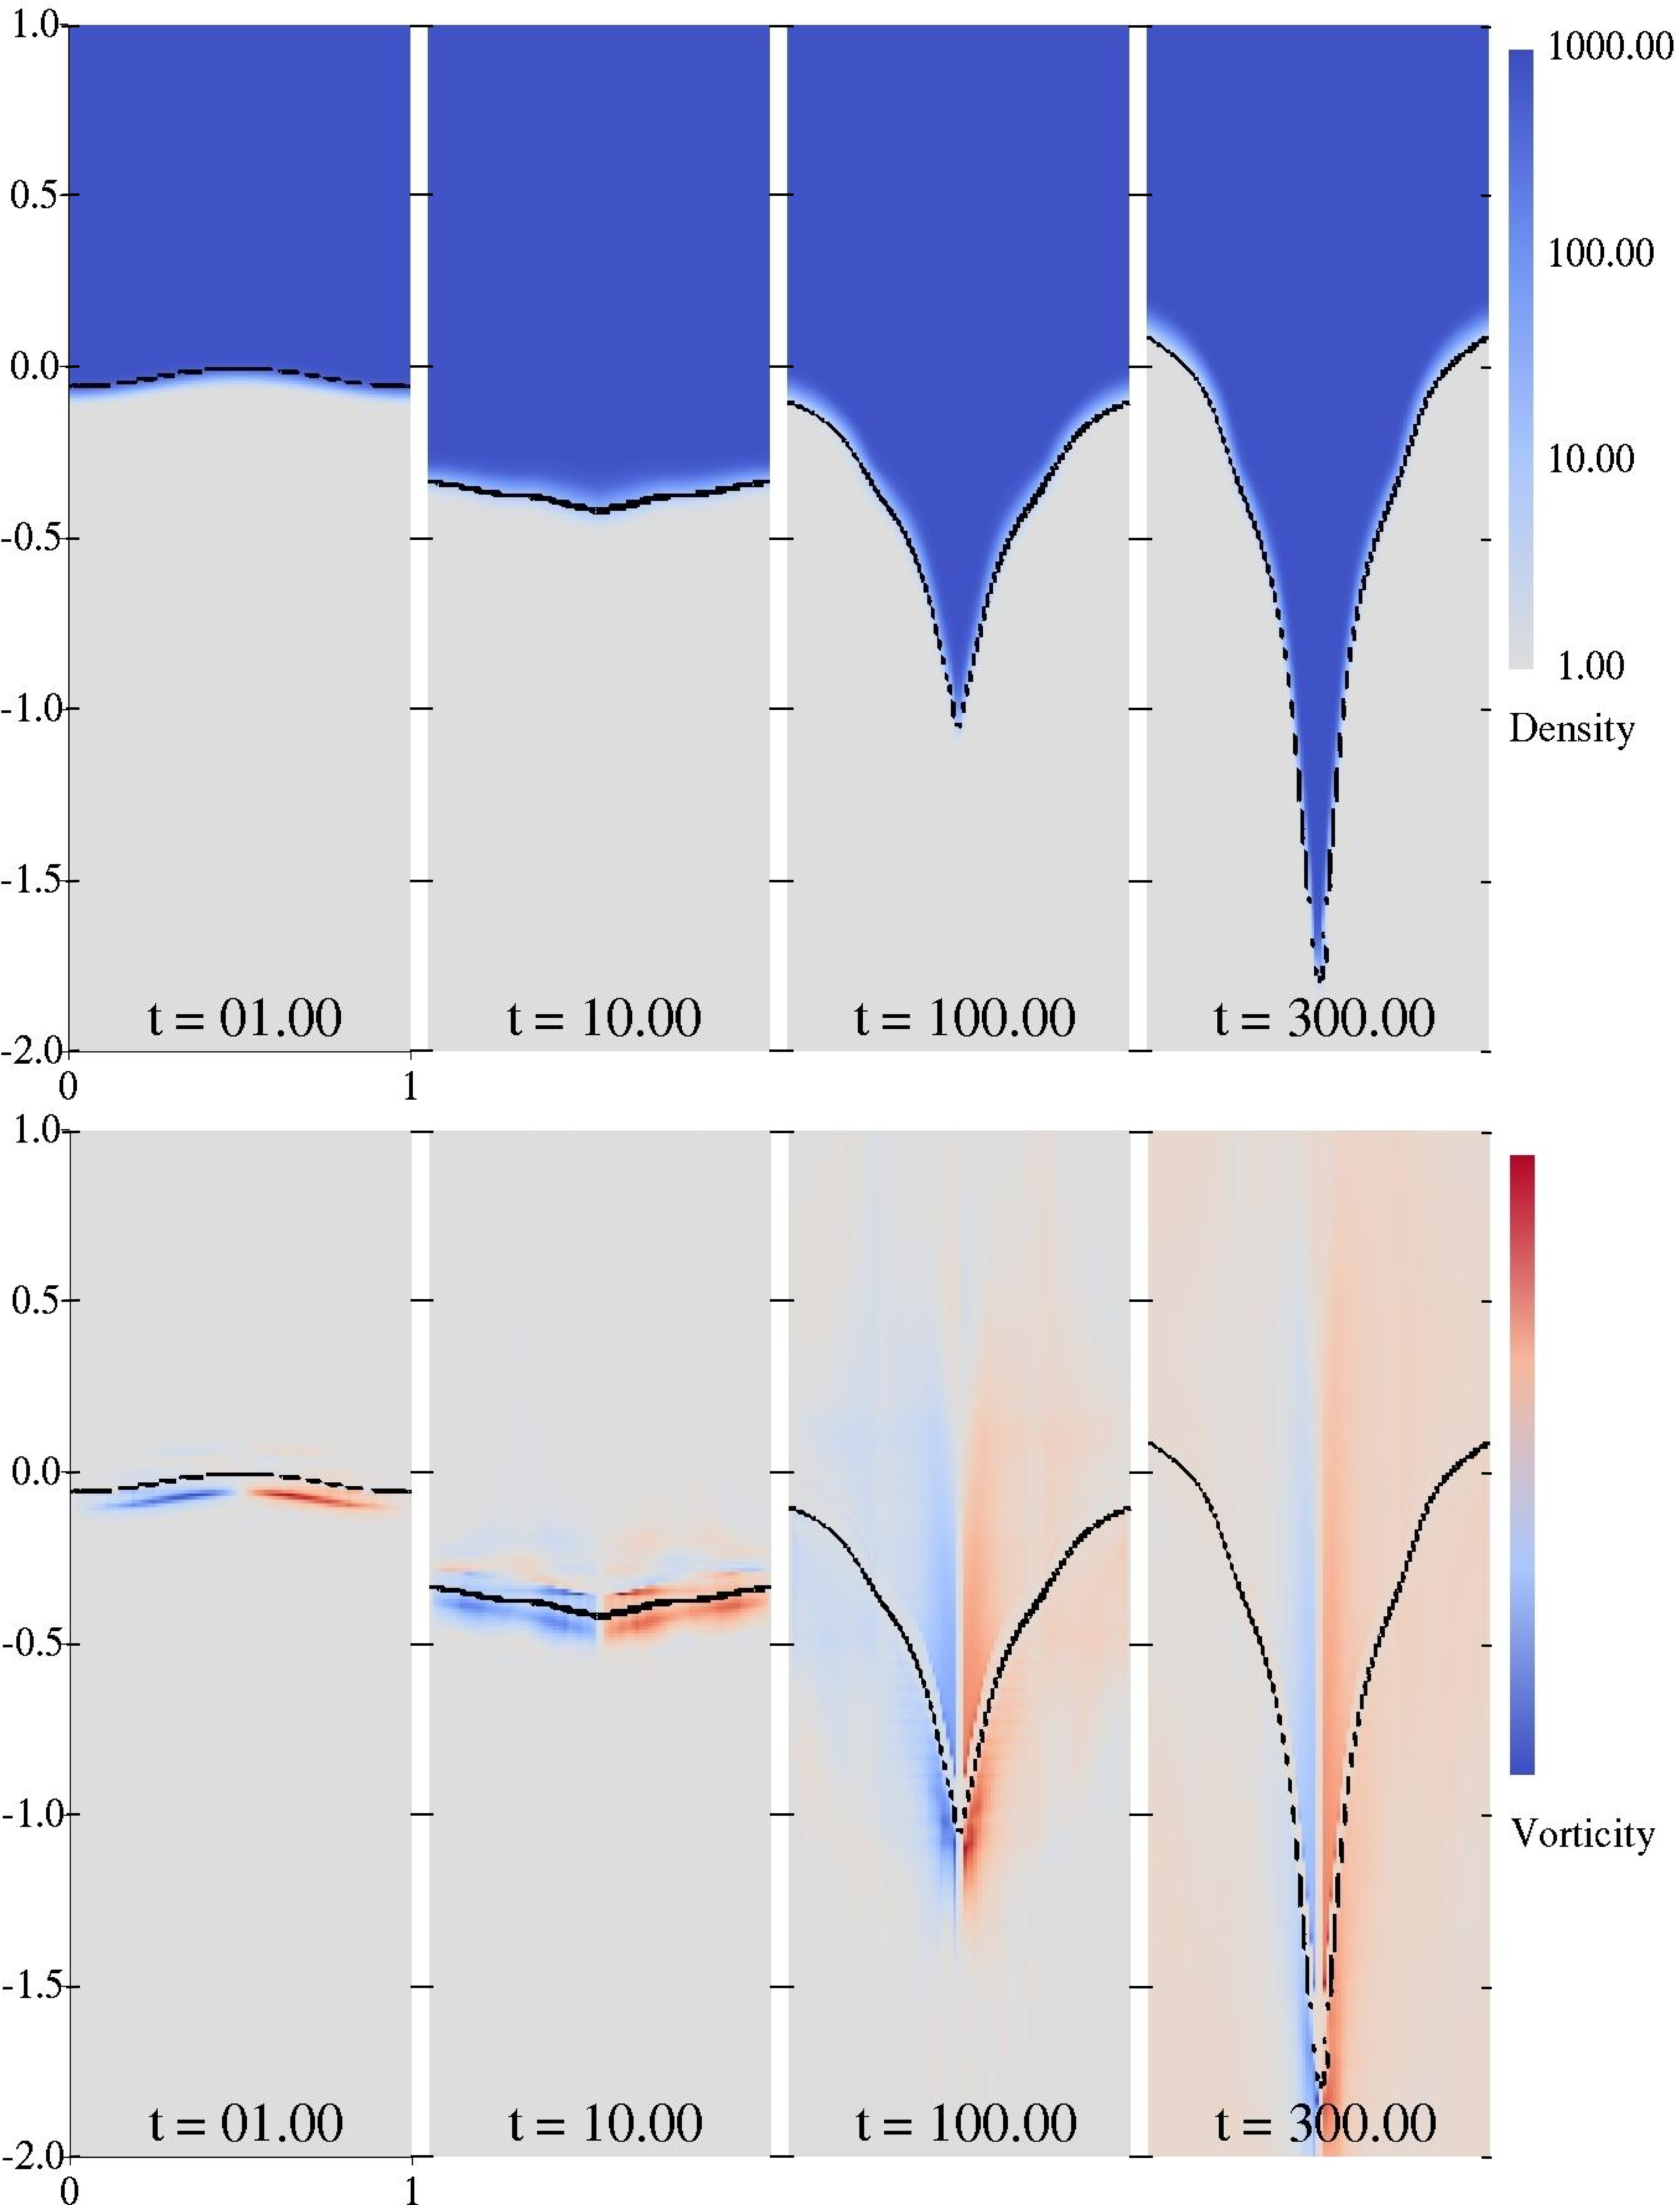
\includegraphics[width=0.9\textwidth]{./figs/lung_figs/snapshots_t1}
\caption[The evolution of the acoustically perturbed interface and vorticity field]{Surface plots of density (Top) and vorticity (Bottom)
  throughout the evolution of the interface for the $10$ MPa
  trapezoidal wave case. Areas of high density (i.e., water) are
indicated in dark blue. Areas of low density (i.e., air) are indicated
in white.  Positive (counterclockwise) vorticity is indicated in red,
and negative (clockwise) vorticity can be seen in blue.}
  \label{fig:interface_snapshots}
\end{figure}
%
\begin{figure}[h] 
  \centering
  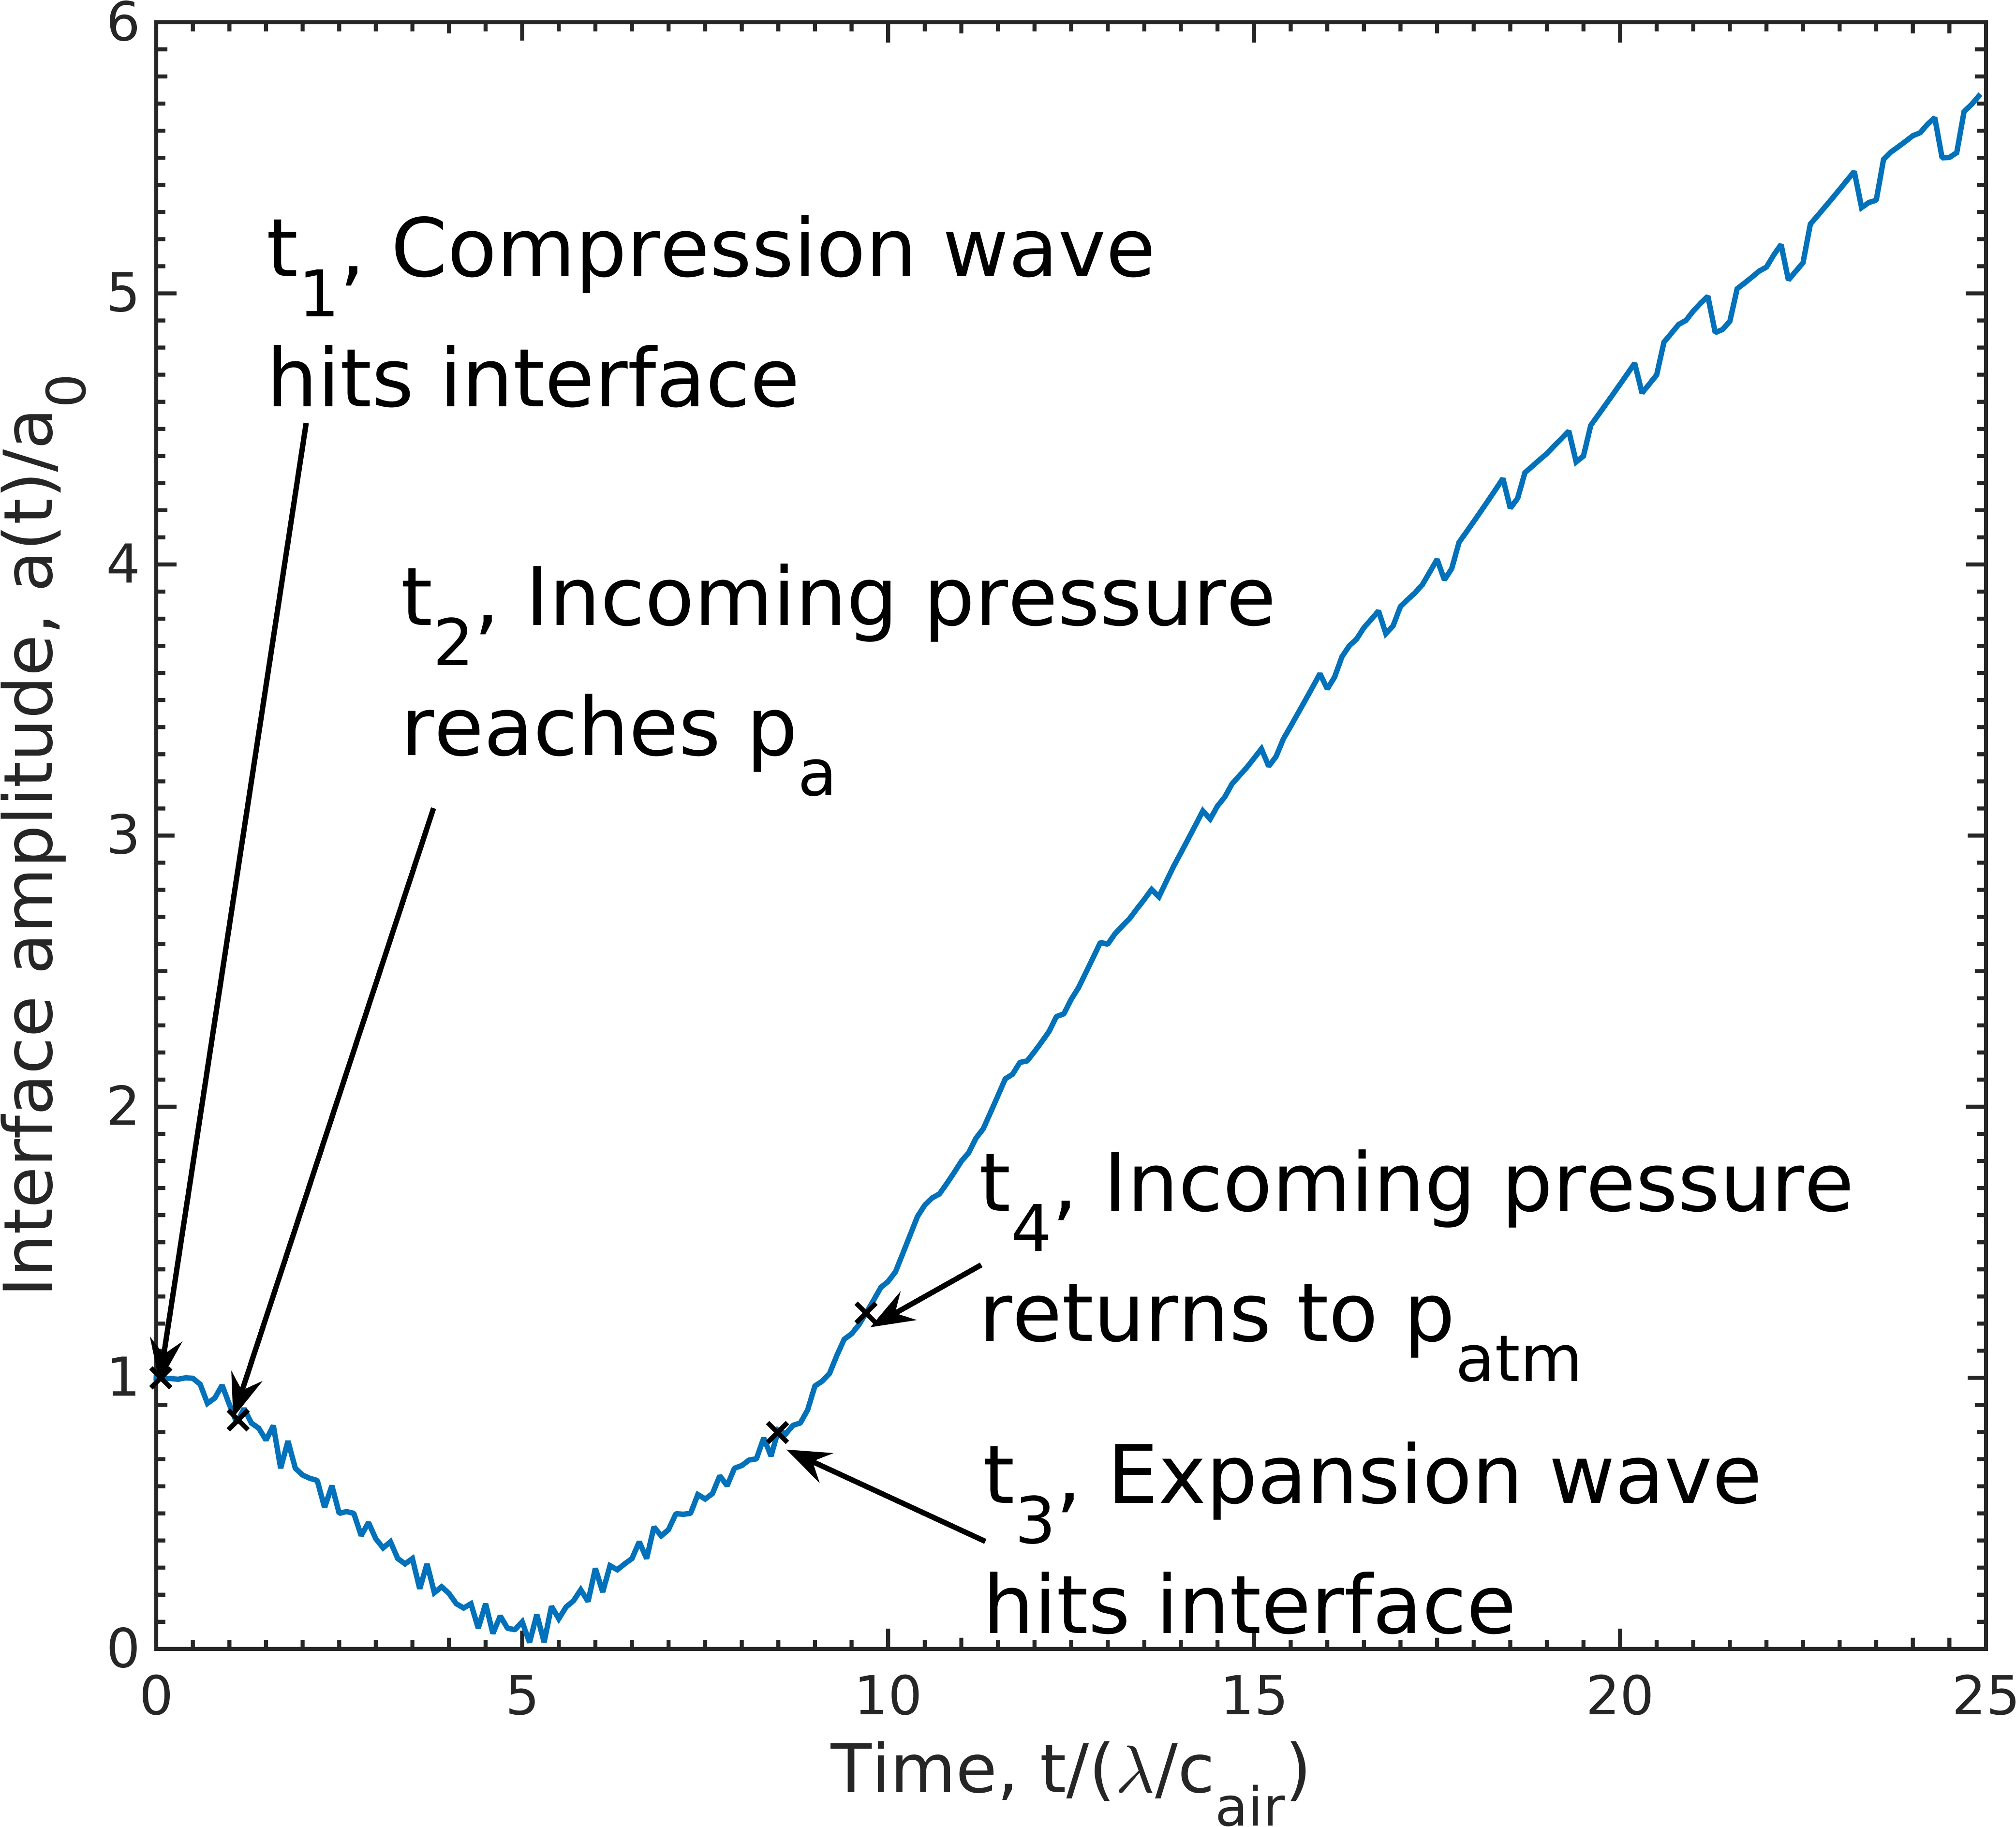
\includegraphics[width=0.48\textwidth]{./figs/lung_figs/trapz10_intf_schematic}
  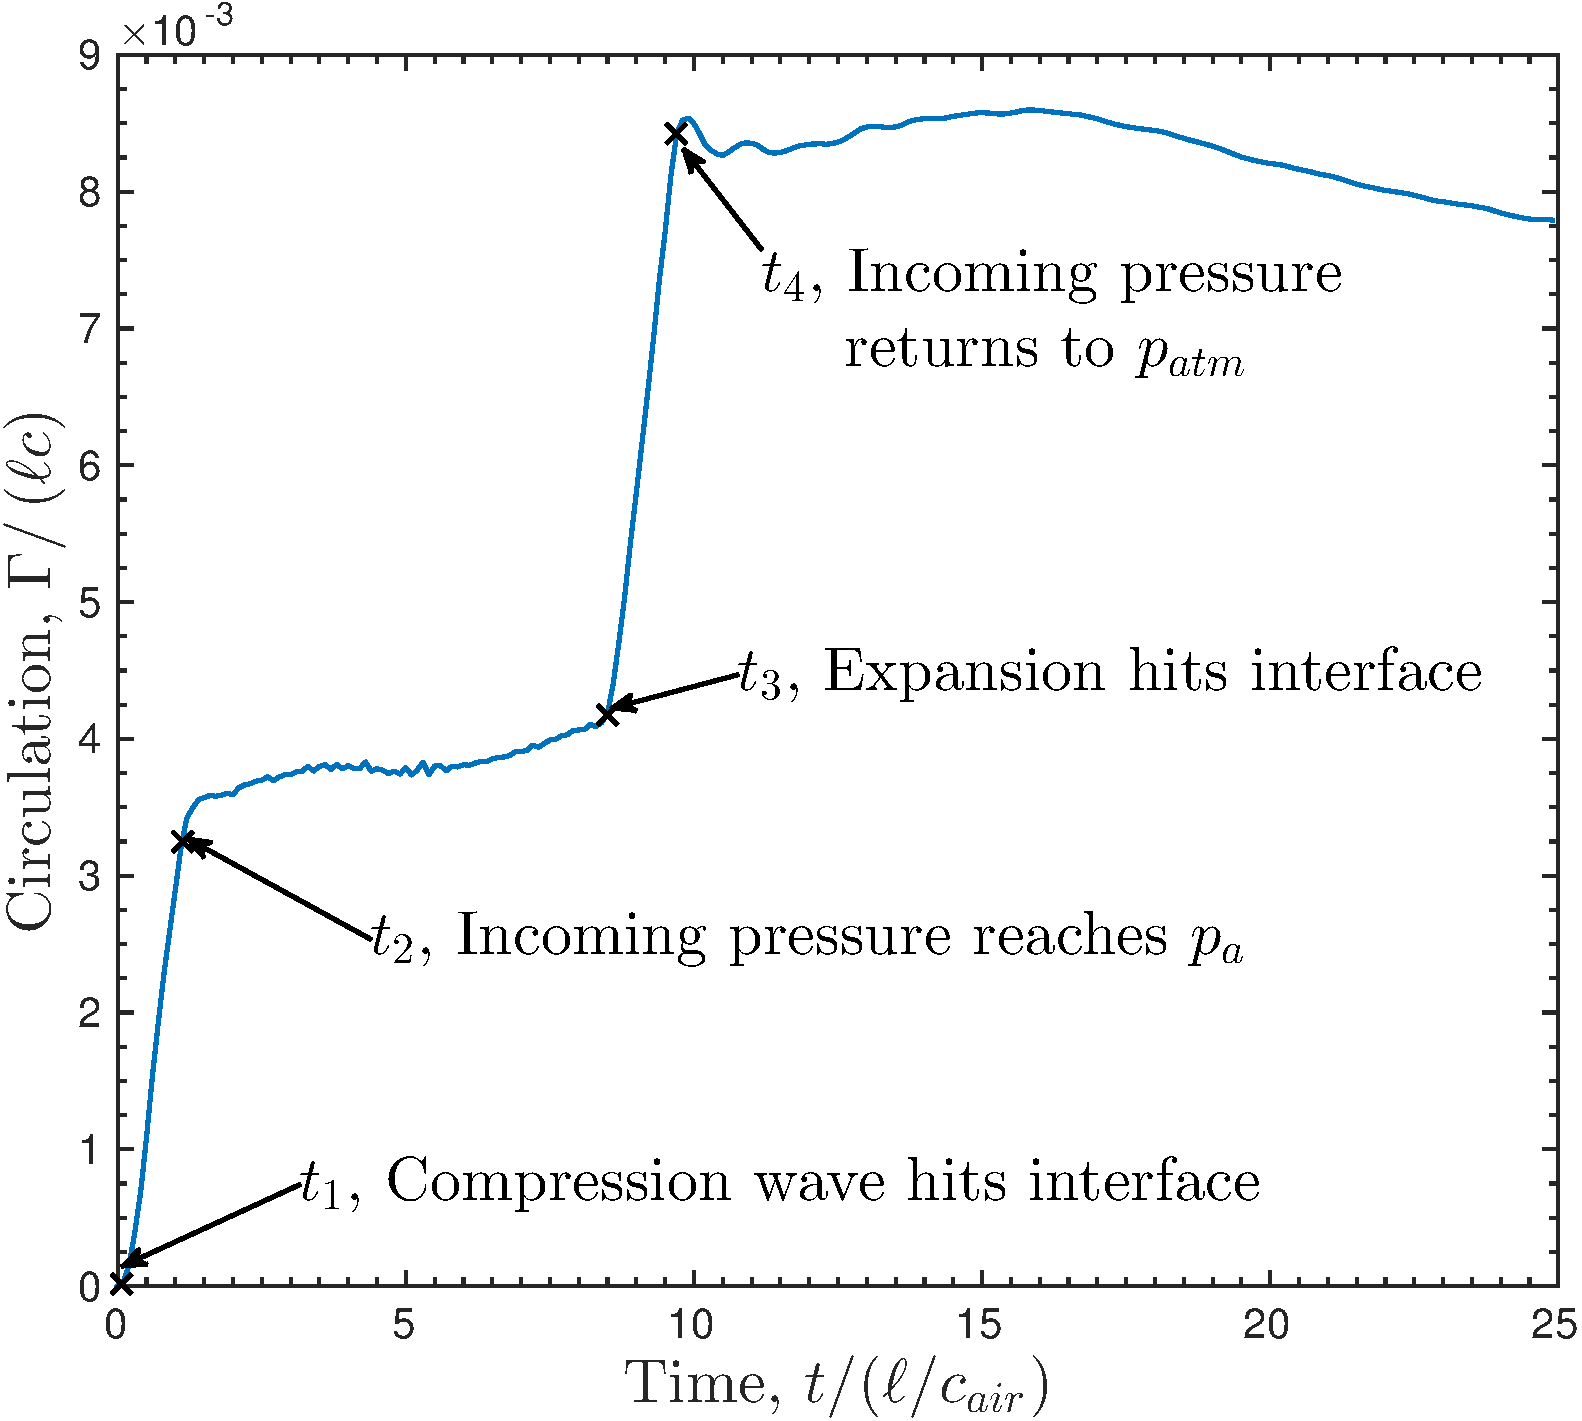
\includegraphics[width=0.48\textwidth]{./figs/lung_figs/trapz10_circ_schematic}
  \caption[The interface amplitude and circulation histories for the $10$ MPa trapezoidal wave]{The interface amplitude (left) and circulation (right)
    histories corresponding to the $10$ MPa trapezoidal waves are
    shown for $t\leq25$. Indicated times, $t_{1-4}$, are the times at
    which different stages of the incoming trapezoidal pressure wave
    shown in Figure \ref{fig:p0} first encounter the interface.}
  \label{fig:trapz10_circ_interface}
\end{figure}
%
\subsubsection{Dependence on wave amplitude}%
\label{subsubsec:usbe_lung_amplitude_dependence}%
To illustrate the effects of varying the trapezoidal wave amplitude,
while keeping the duration of each wave feature constant, we show
interface amplitudes and half-domain circulation histories for
$p_a=1$, $5$, and $10$ MPa trapezoidal waves. In Figure
\ref{fig:trapz_circ_interface_early}, we look closely at the period
around the wave interaction for $0 \leq t\leq 25$. We note that the
for the $p_a10$ MPa case, the phase reversal of the interface happened
around $t=5.0$, which is about haft the time it took for this to occur
for the for the $p_a=5$ MPa case. The $p_a1$ MPa case, the evolution
of the interface is sufficiently slow as to not phase invert during
the period shown. For each wave amplitude, the circulation is
normalized by the $p_a$ to show that the circulation generated by the
interface-compression wave interaction, $0^+<t<scales<0.12$, increases
linearly with $p_a$. To show the longer term effects of varying
amplitude and show the late time behavior of the interface, defined as
the behavior significantly after the acoustic waves have left the
domain, Figure \ref{fig:trapz_circ_interface_loglog} shows the
interface amplitude and half-domain circulation histories for
$0 \leq t\leq 500$ as functions of time for $5$ and $10$ MPa
trapezoidal waves impinging on the interface. Here, the interface
amplitude is plotted on logarithmically-scaled axes. From scaling law
\eqref{eq:intf_circ_scaling} we expect that for purely circulation
driven interface growth, $a(t)$ will grow with $\sqrt{t}$, which is
shown by dashed lines of corresponding colors. For the $10$ MPa wave
case the slope of the observed growth appears to grow as $t^{0.6}$.
Longer time simulations will be used to see if this settles to the
expected $\sqrt(t)$ growth. Note that results for the $1$ MPa
trapezoidal wave were not included because the slow evolution of the
interface made the computation prohibitively expensive.
%
\begin{figure}[h] 
  \centering
  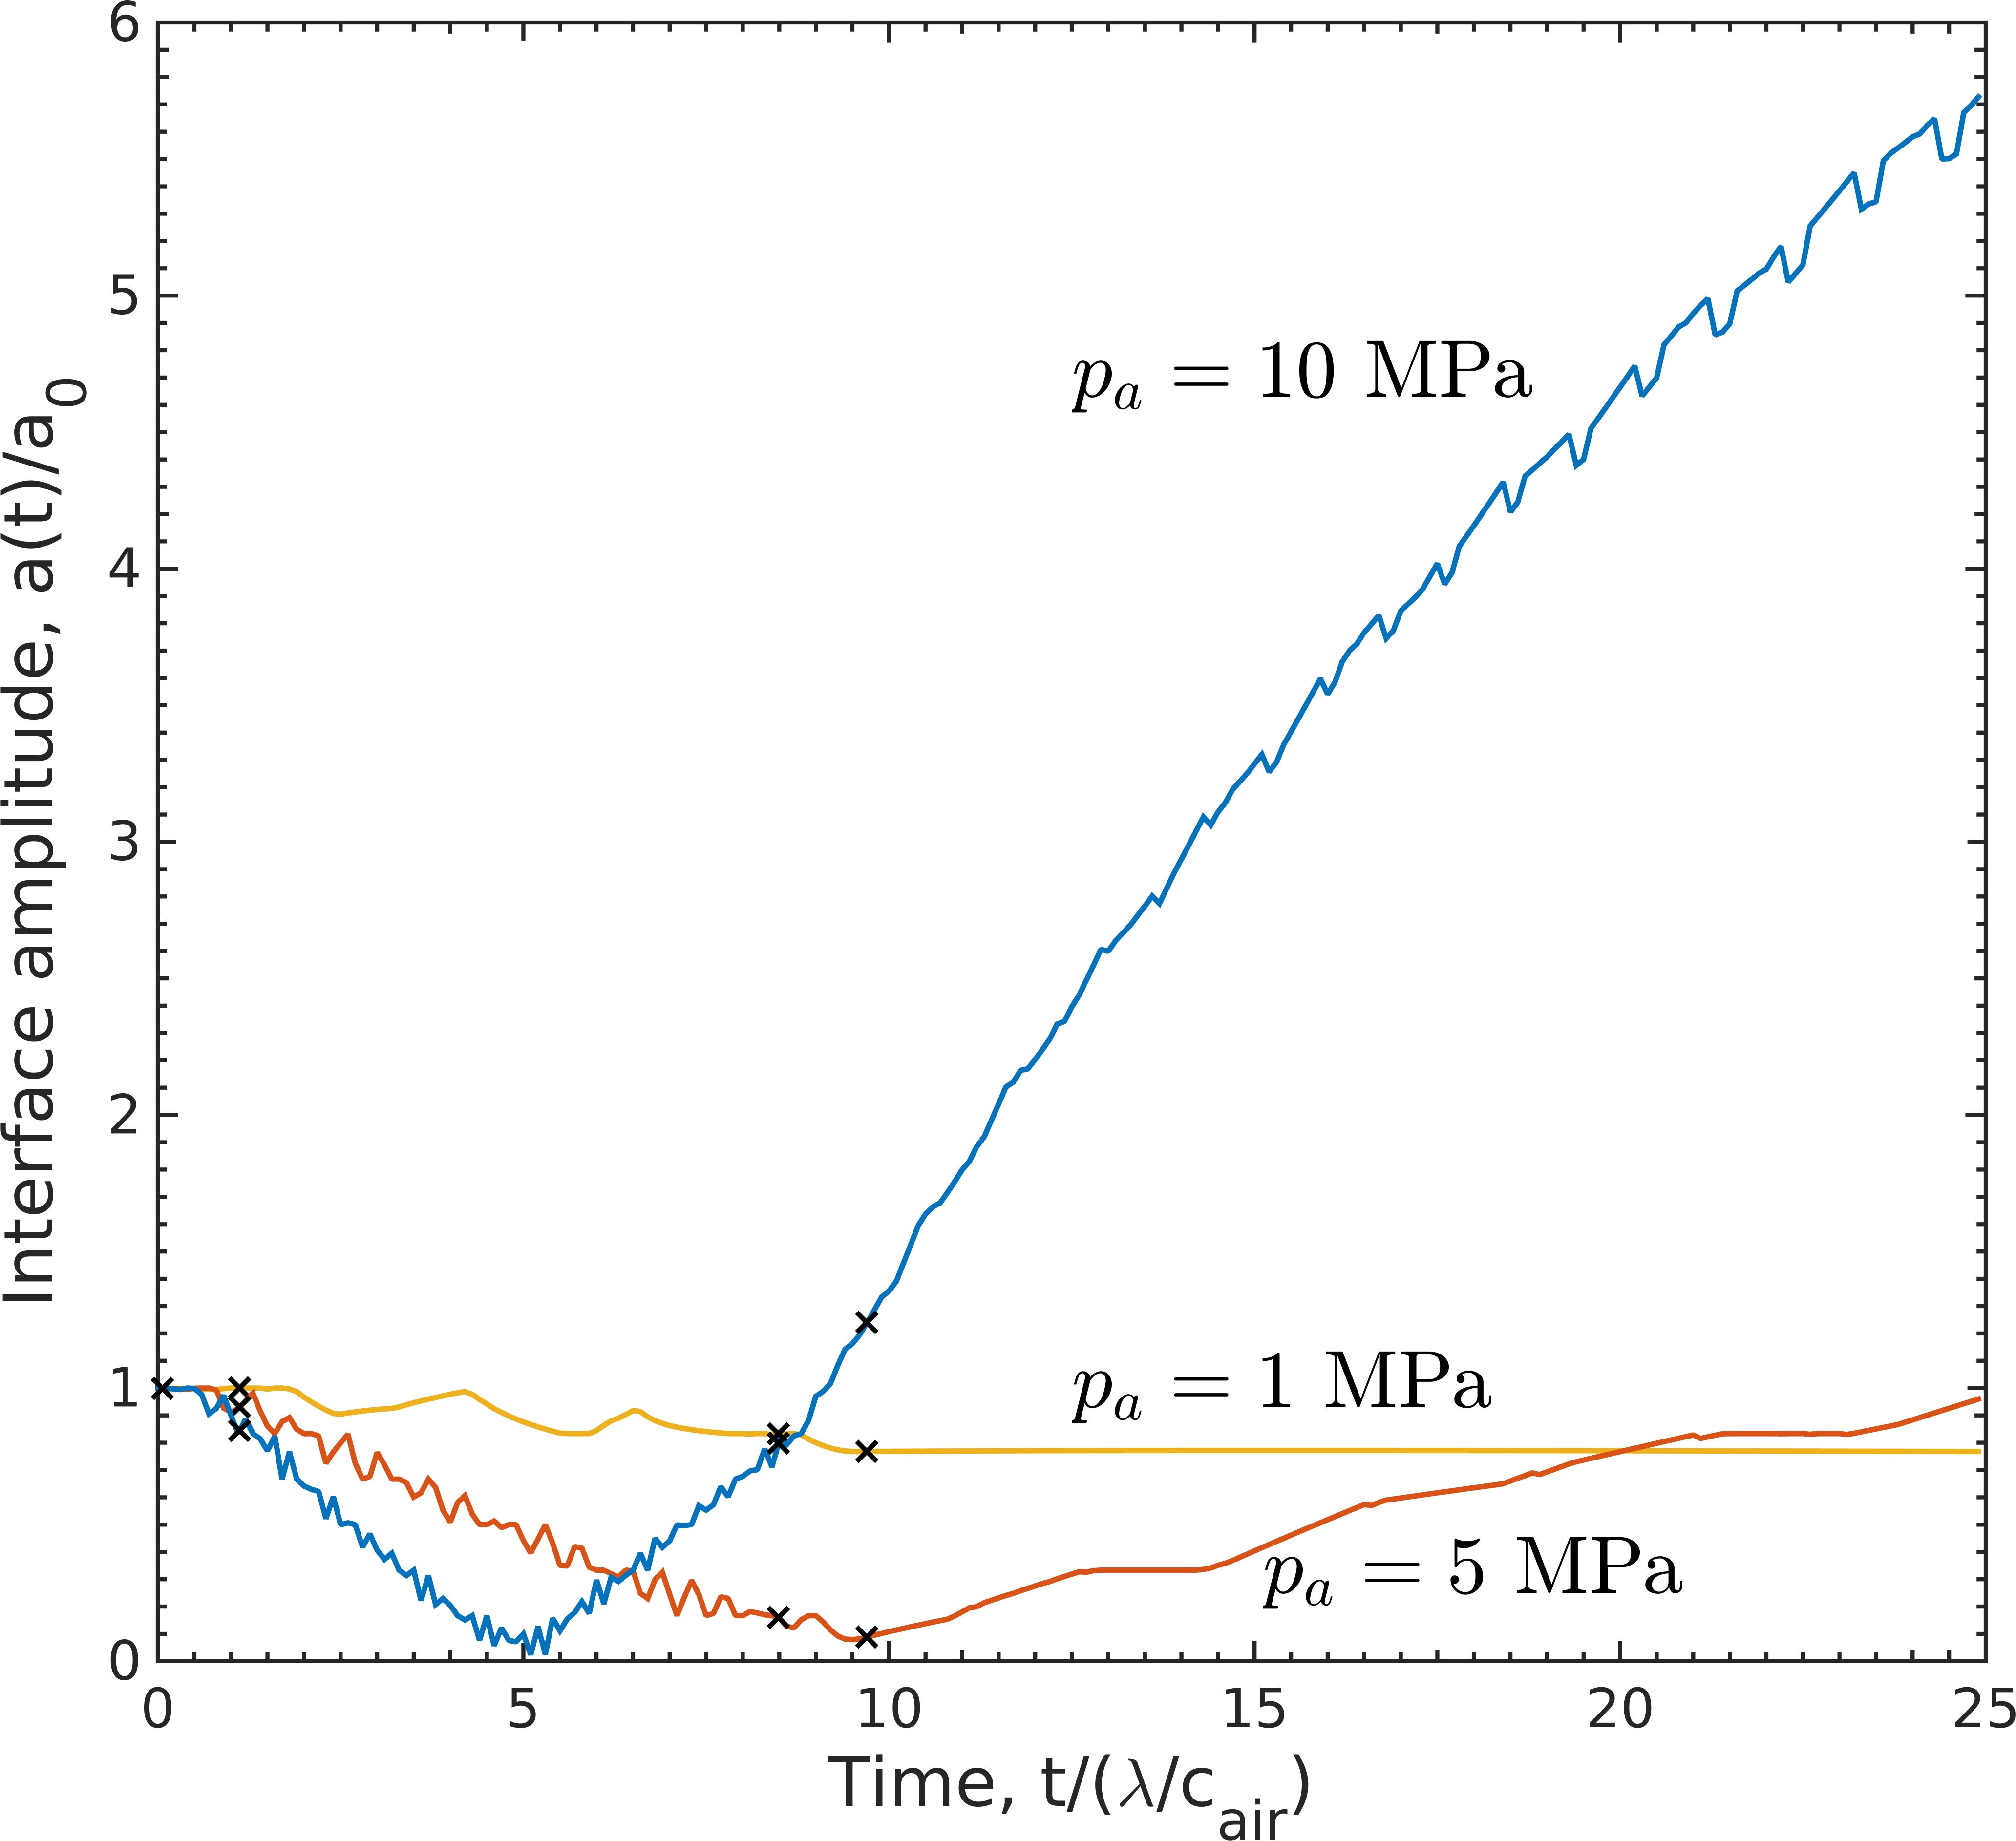
\includegraphics[width=0.48\textwidth]{./figs/lung_figs/interface_multi-amp_norm}
  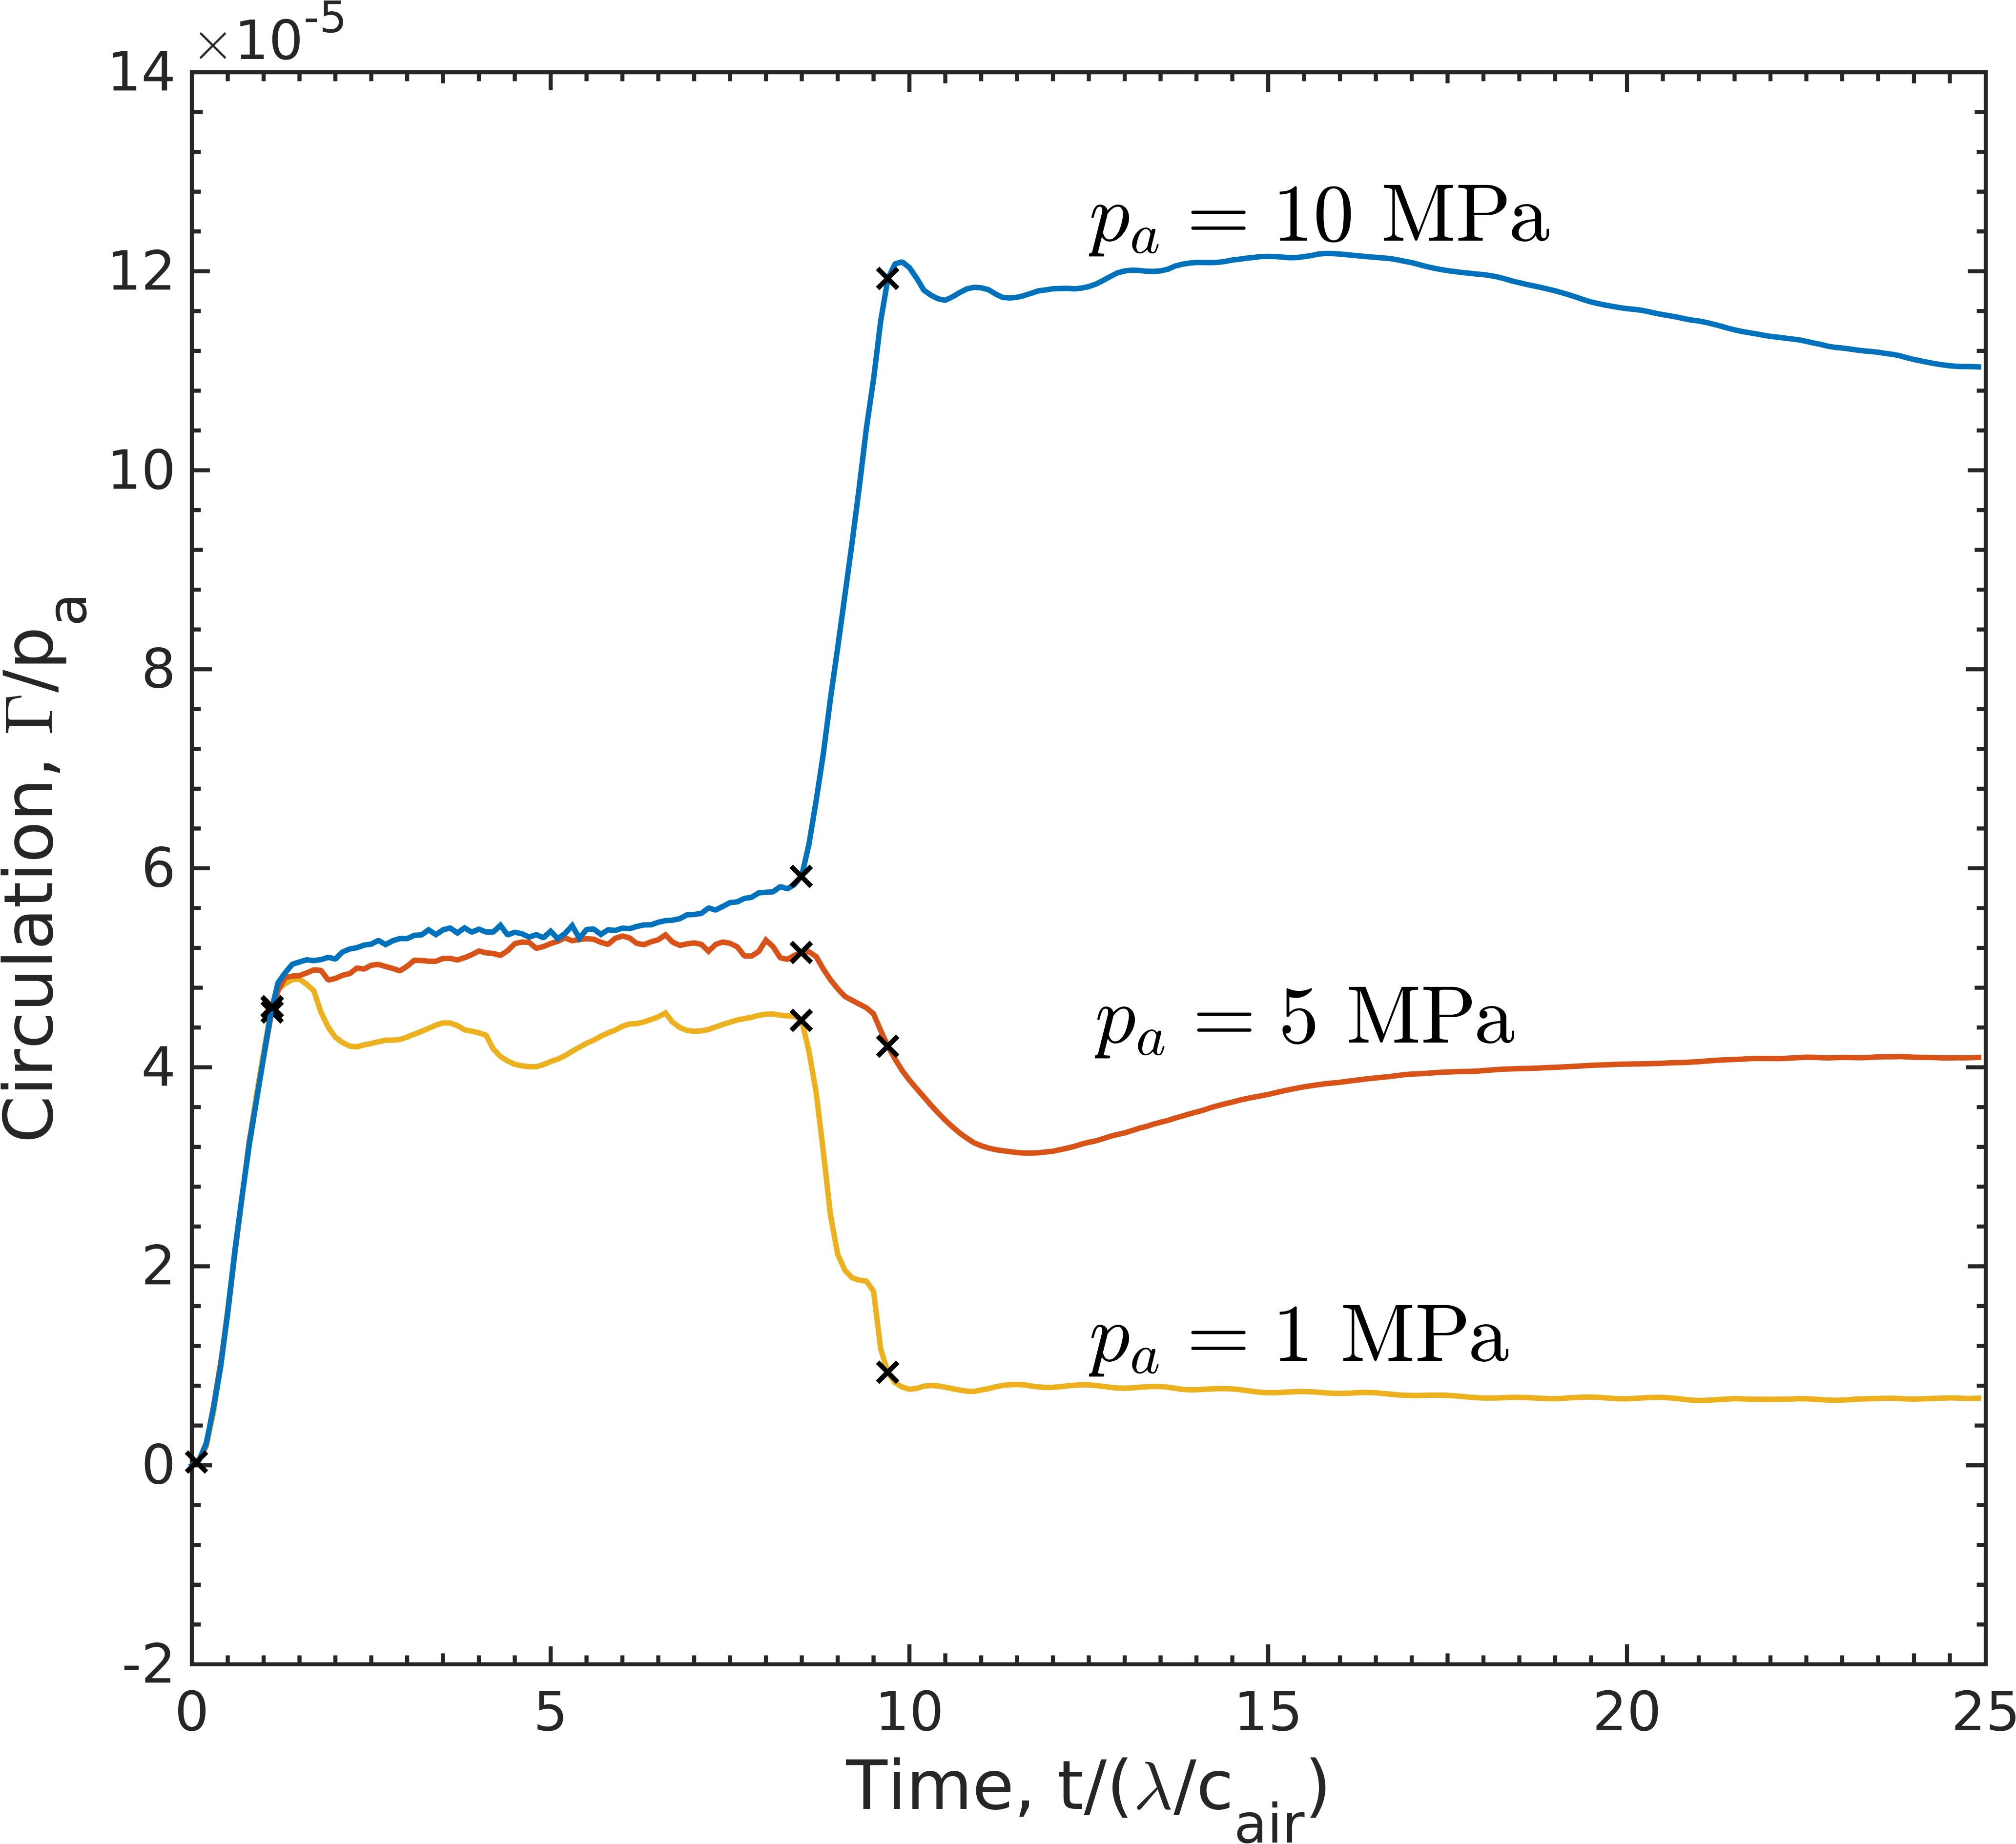
\includegraphics[width=0.48\textwidth]{./figs/lung_figs/circulation_multi-amp_norm}
  \caption[The interface and circulation dependence on wave amplitude at early time]{The interface amplitude (left) and circulation (right)
    histories corresponding to the $1$(yellow), $5$(orange), and
    $10$(blue) MPa trapezoidal waves are shown for $t\leq 25$. The
    circulation history is normalized by the acoustic amplitude of the
    incoming wave to illustrate that circulation deposition by the
    compression wave scales linearly with $p_a$ }
  \label{fig:trapz_circ_interface_early}
\end{figure}
%
\begin{figure}[h] 
  \centering
  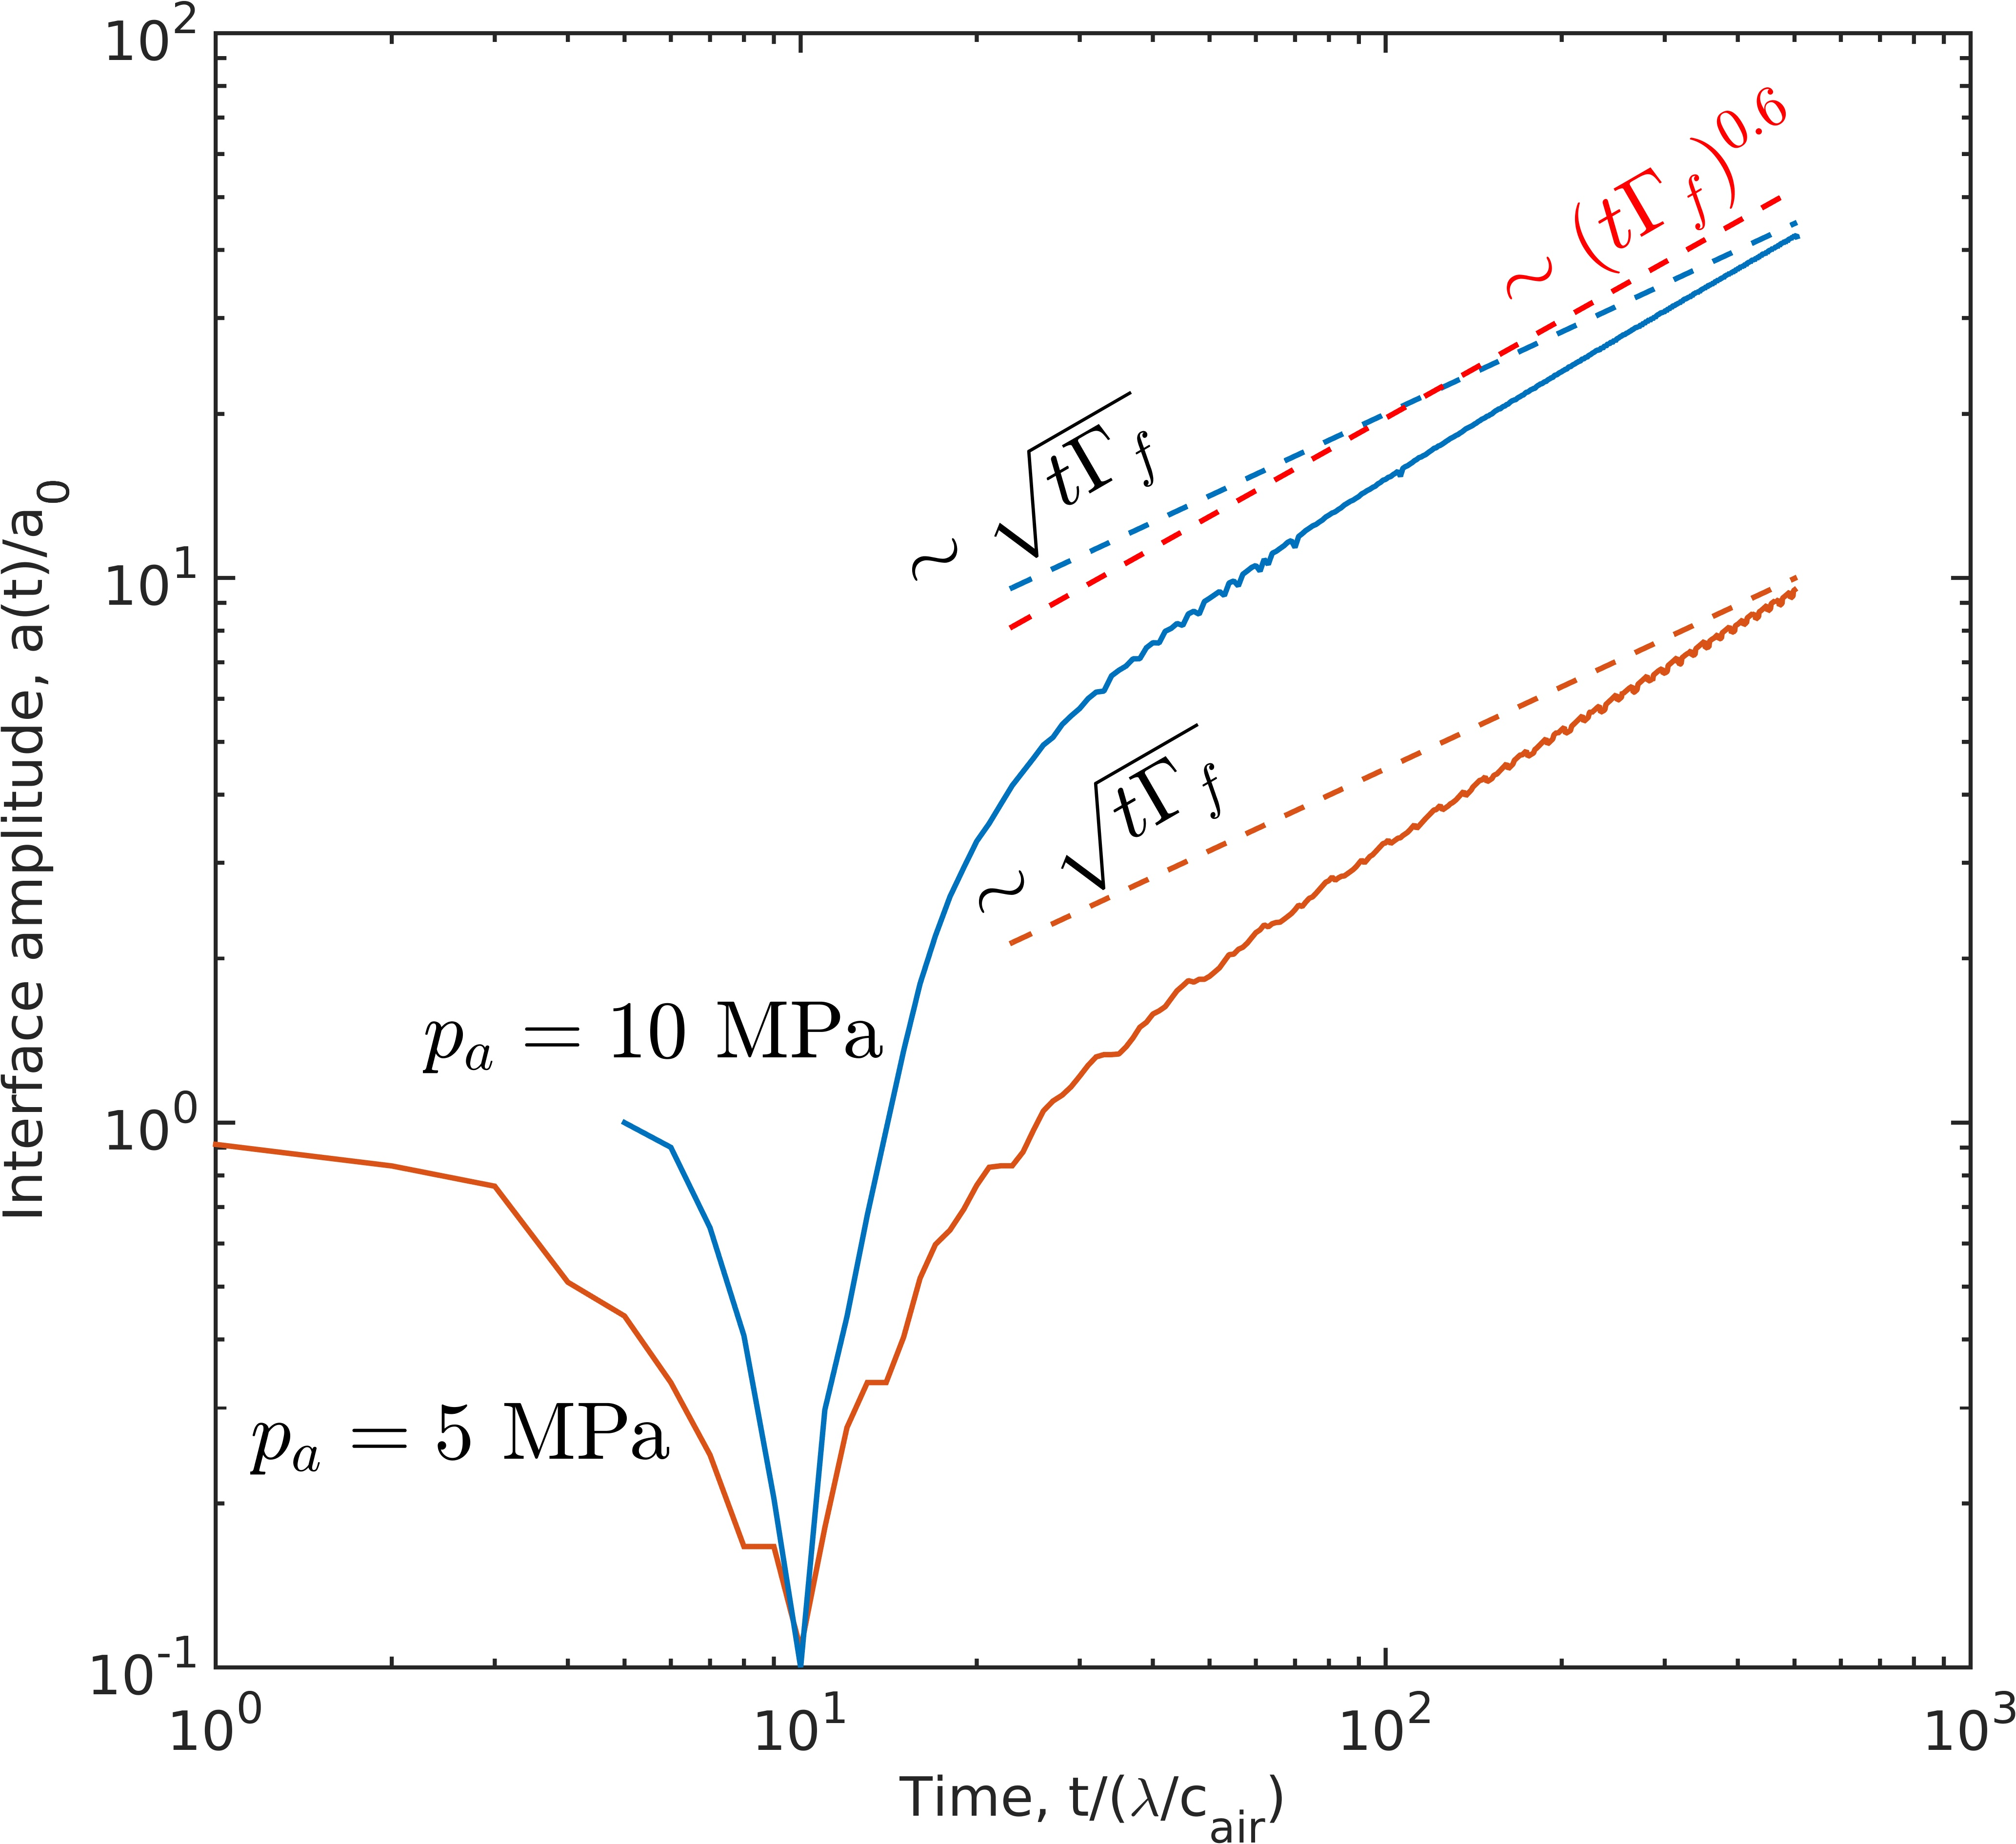
\includegraphics[width=0.48\textwidth]{./figs/lung_figs/interface_multi-amp_loglog_roe_extra}
  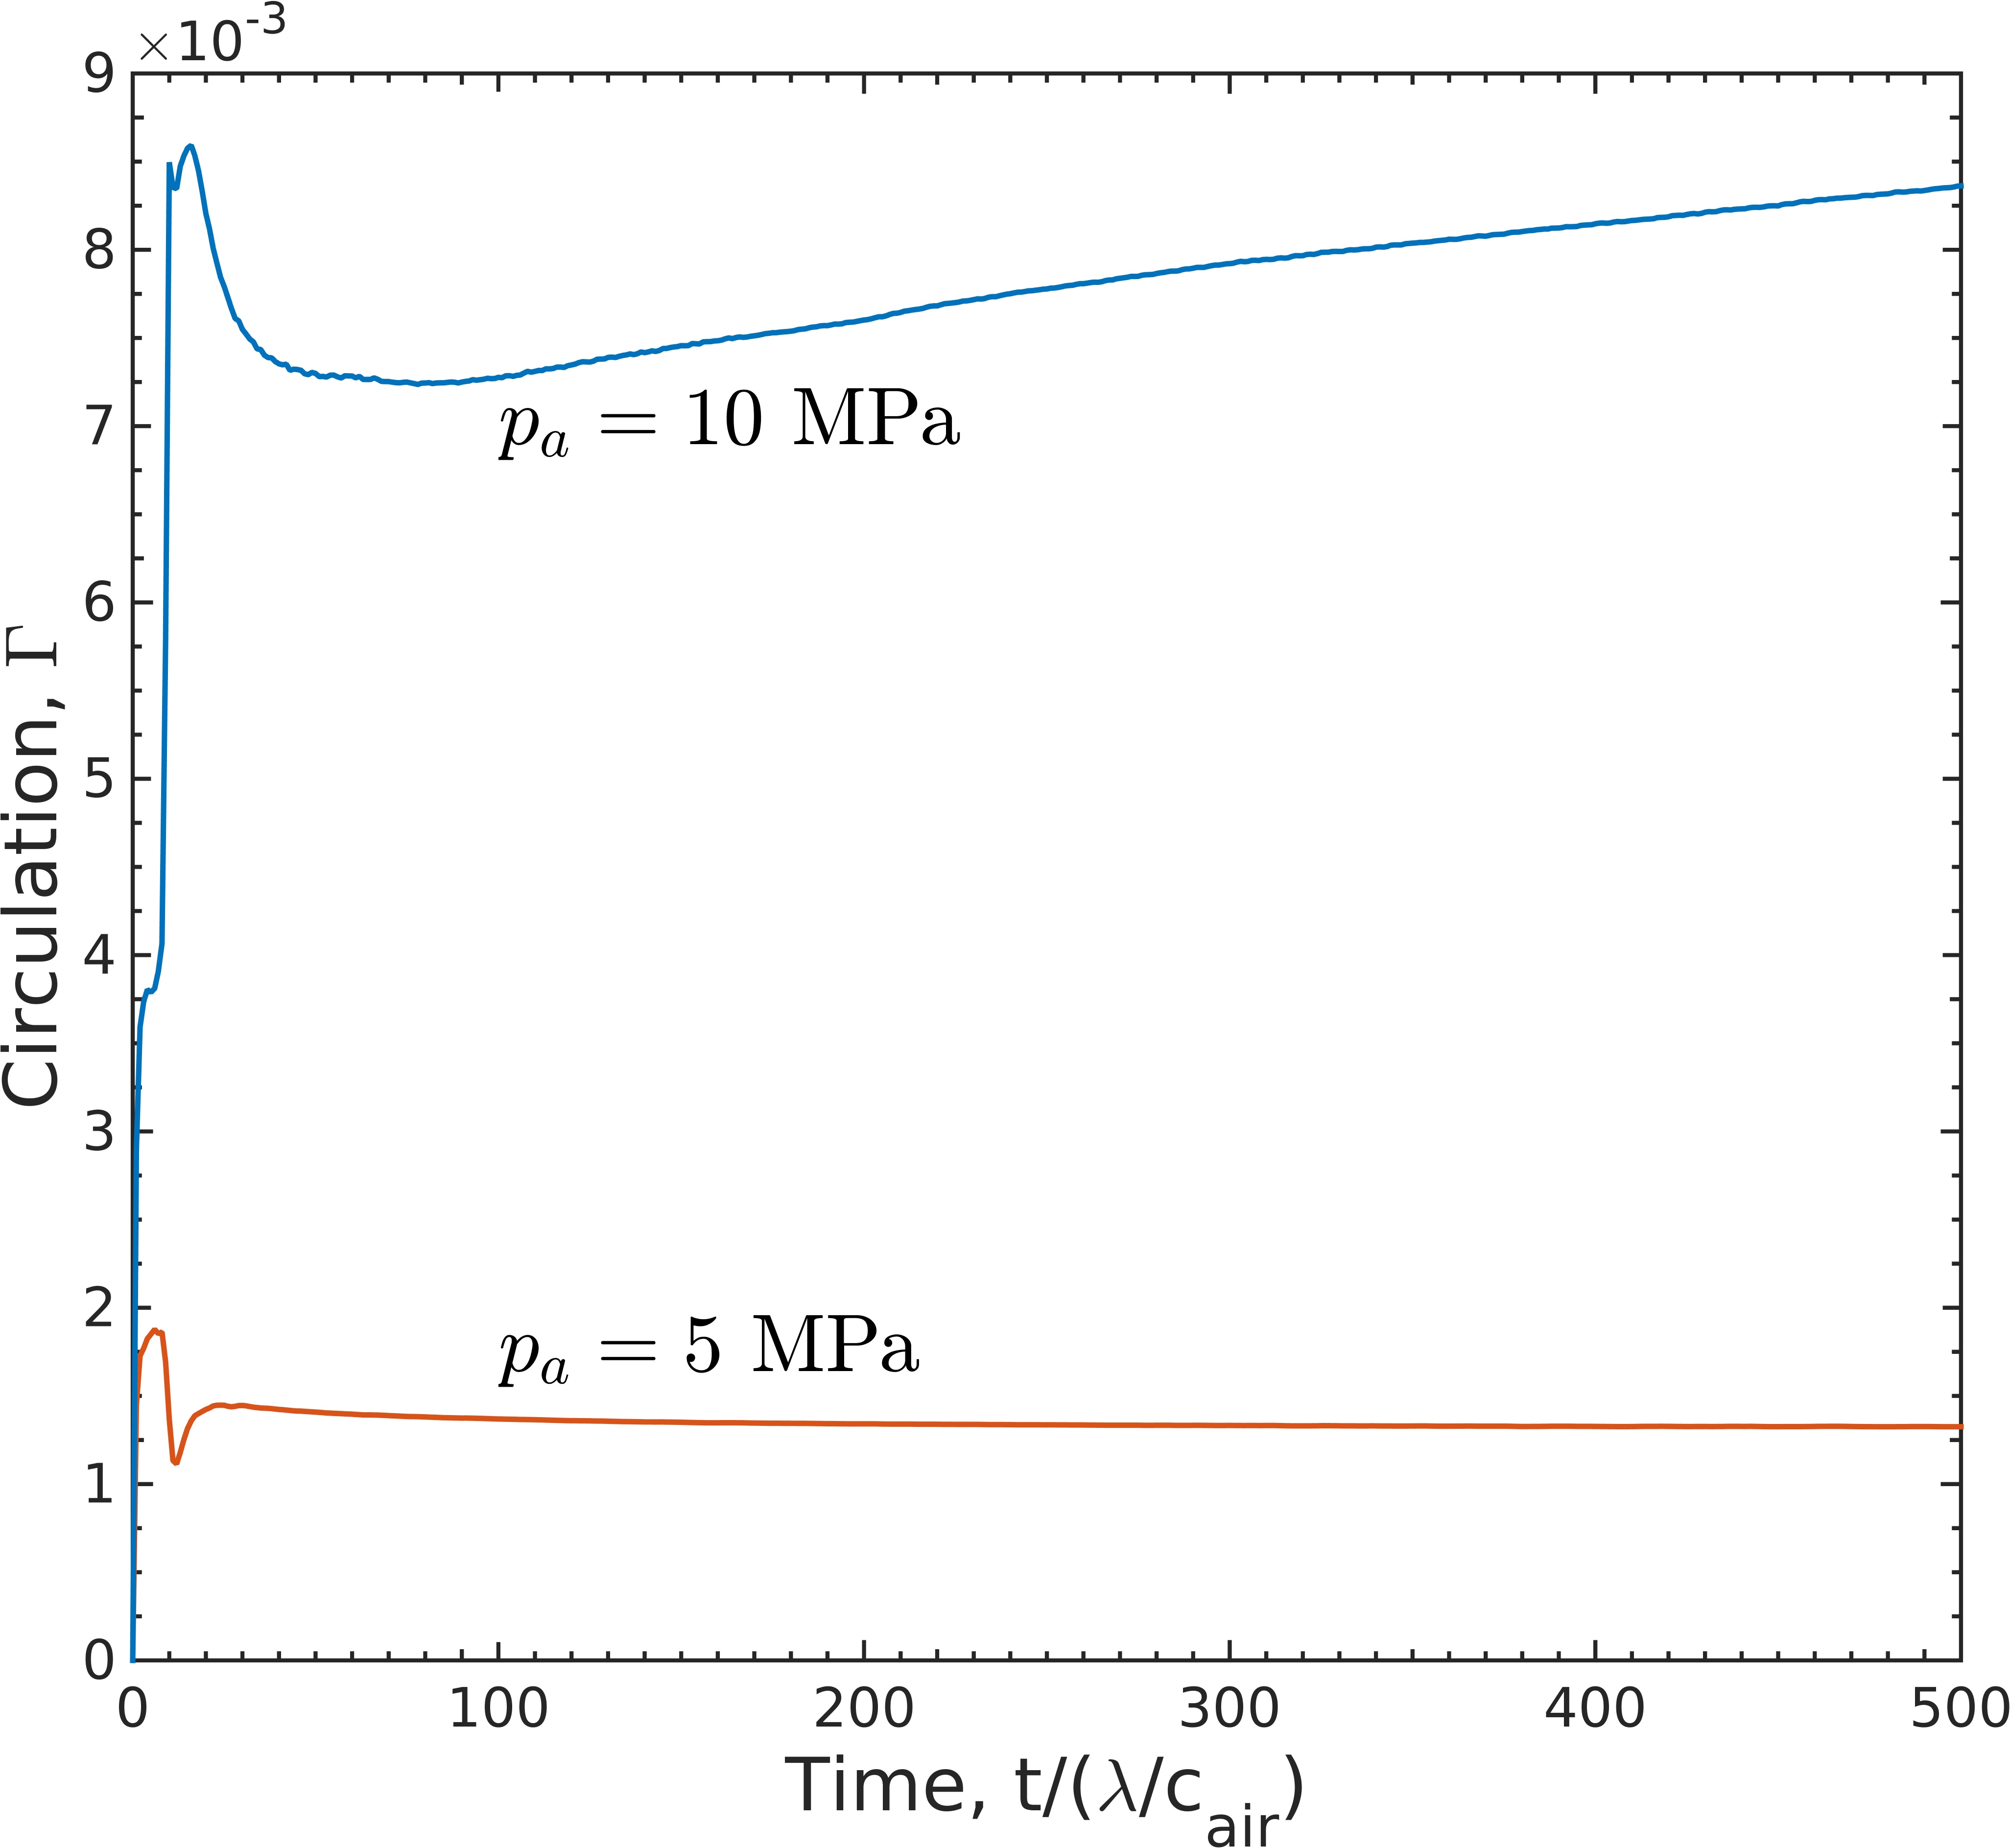
\includegraphics[width=0.48\textwidth]{./figs/lung_figs/circulation_multi-amp2_roe}
  \caption[The interface and circulation dependence on wave amplitude
  at long time]{The interface amplitude (left) and circulation (right)
    histories corresponding to the $5$(orange) and $10$(blue) MPa
    trapezoidal waves are shown for $t\leq 500$. To appropriately
    compare late time dynamics, time has been offset in the interface
    amplitude history such that the phase reversal appears to occur
    simultaneously in both simulations. Dashed lines of the same color
    are used to demonstrate the expected slope of pure circulation
    driven interface growth, based on Equation
    \eqref{eq:intf_circ_scaling}. The red dashed line shows the slope we
    appear to be approaching for the $10$ MPa wave case for the end time.}
  \label{fig:trapz_circ_interface_loglog}
\end{figure}
%
\subsubsection{Circulation and vorticity dynamics}
We observe that the wave deposits a sheet of vorticity along the
interface that moves with the interface in time. Figure
\ref{fig:trapz_ddt_circ} shows a surface plot of vorticity in the
region of the domain around the interface for the $10$ Mpa trapezoidal
wave case, at $t=0.6$, during the middle of the interface-compression
wave interaction (Left). Not shown is the rest of the domain, where
vorticity was relatively insignificant. The vorticity is antisymmetric
across the $x=0.5$ center line. To analyze the physical mechanisms
generating the vorticity, we plot each term of the circulation
generation equation \eqref{eq:circulation_generation} during the
period around the compression wave-interface interaction. Near the end
of the interaction at $t=1.0$,
$\left(\partial \Gamma/\partial t\right)_{advective} =
5.3\,\text{e}{-5}$; %
$\left(\partial \Gamma/\partial t\right)_{compressible} =
-2.7\,\text{e}{-5}$; %
$\left(\partial \Gamma/\partial t\right)_{baroclinic} =
-7.7\,\text{e}{-3}$; %
$\left(\partial \Gamma/\partial t\right)_{total} =
-7.7\,\text{e}{-3}$. %
This result is quantitatively consistent with expected vorticity generation
based on our analysis \eqref{eq:vorticity_comparison}. Furthermore, it
supports our hypothesis that vorticity is primarily baroclinically
generated. 
%
\begin{figure}[h] 
  \centering
  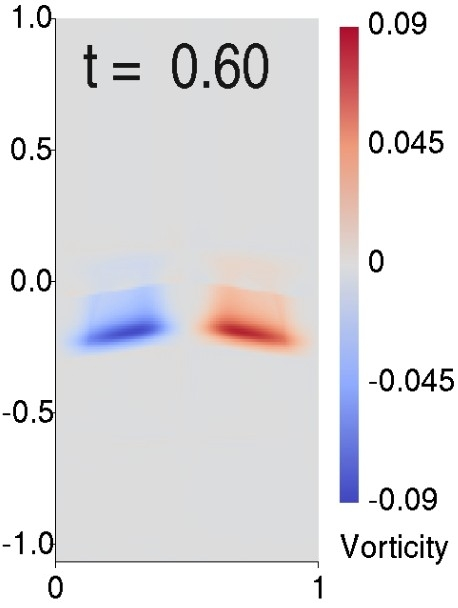
\includegraphics[width=0.35\textwidth]{./figs/lung_figs/vorticity2}
  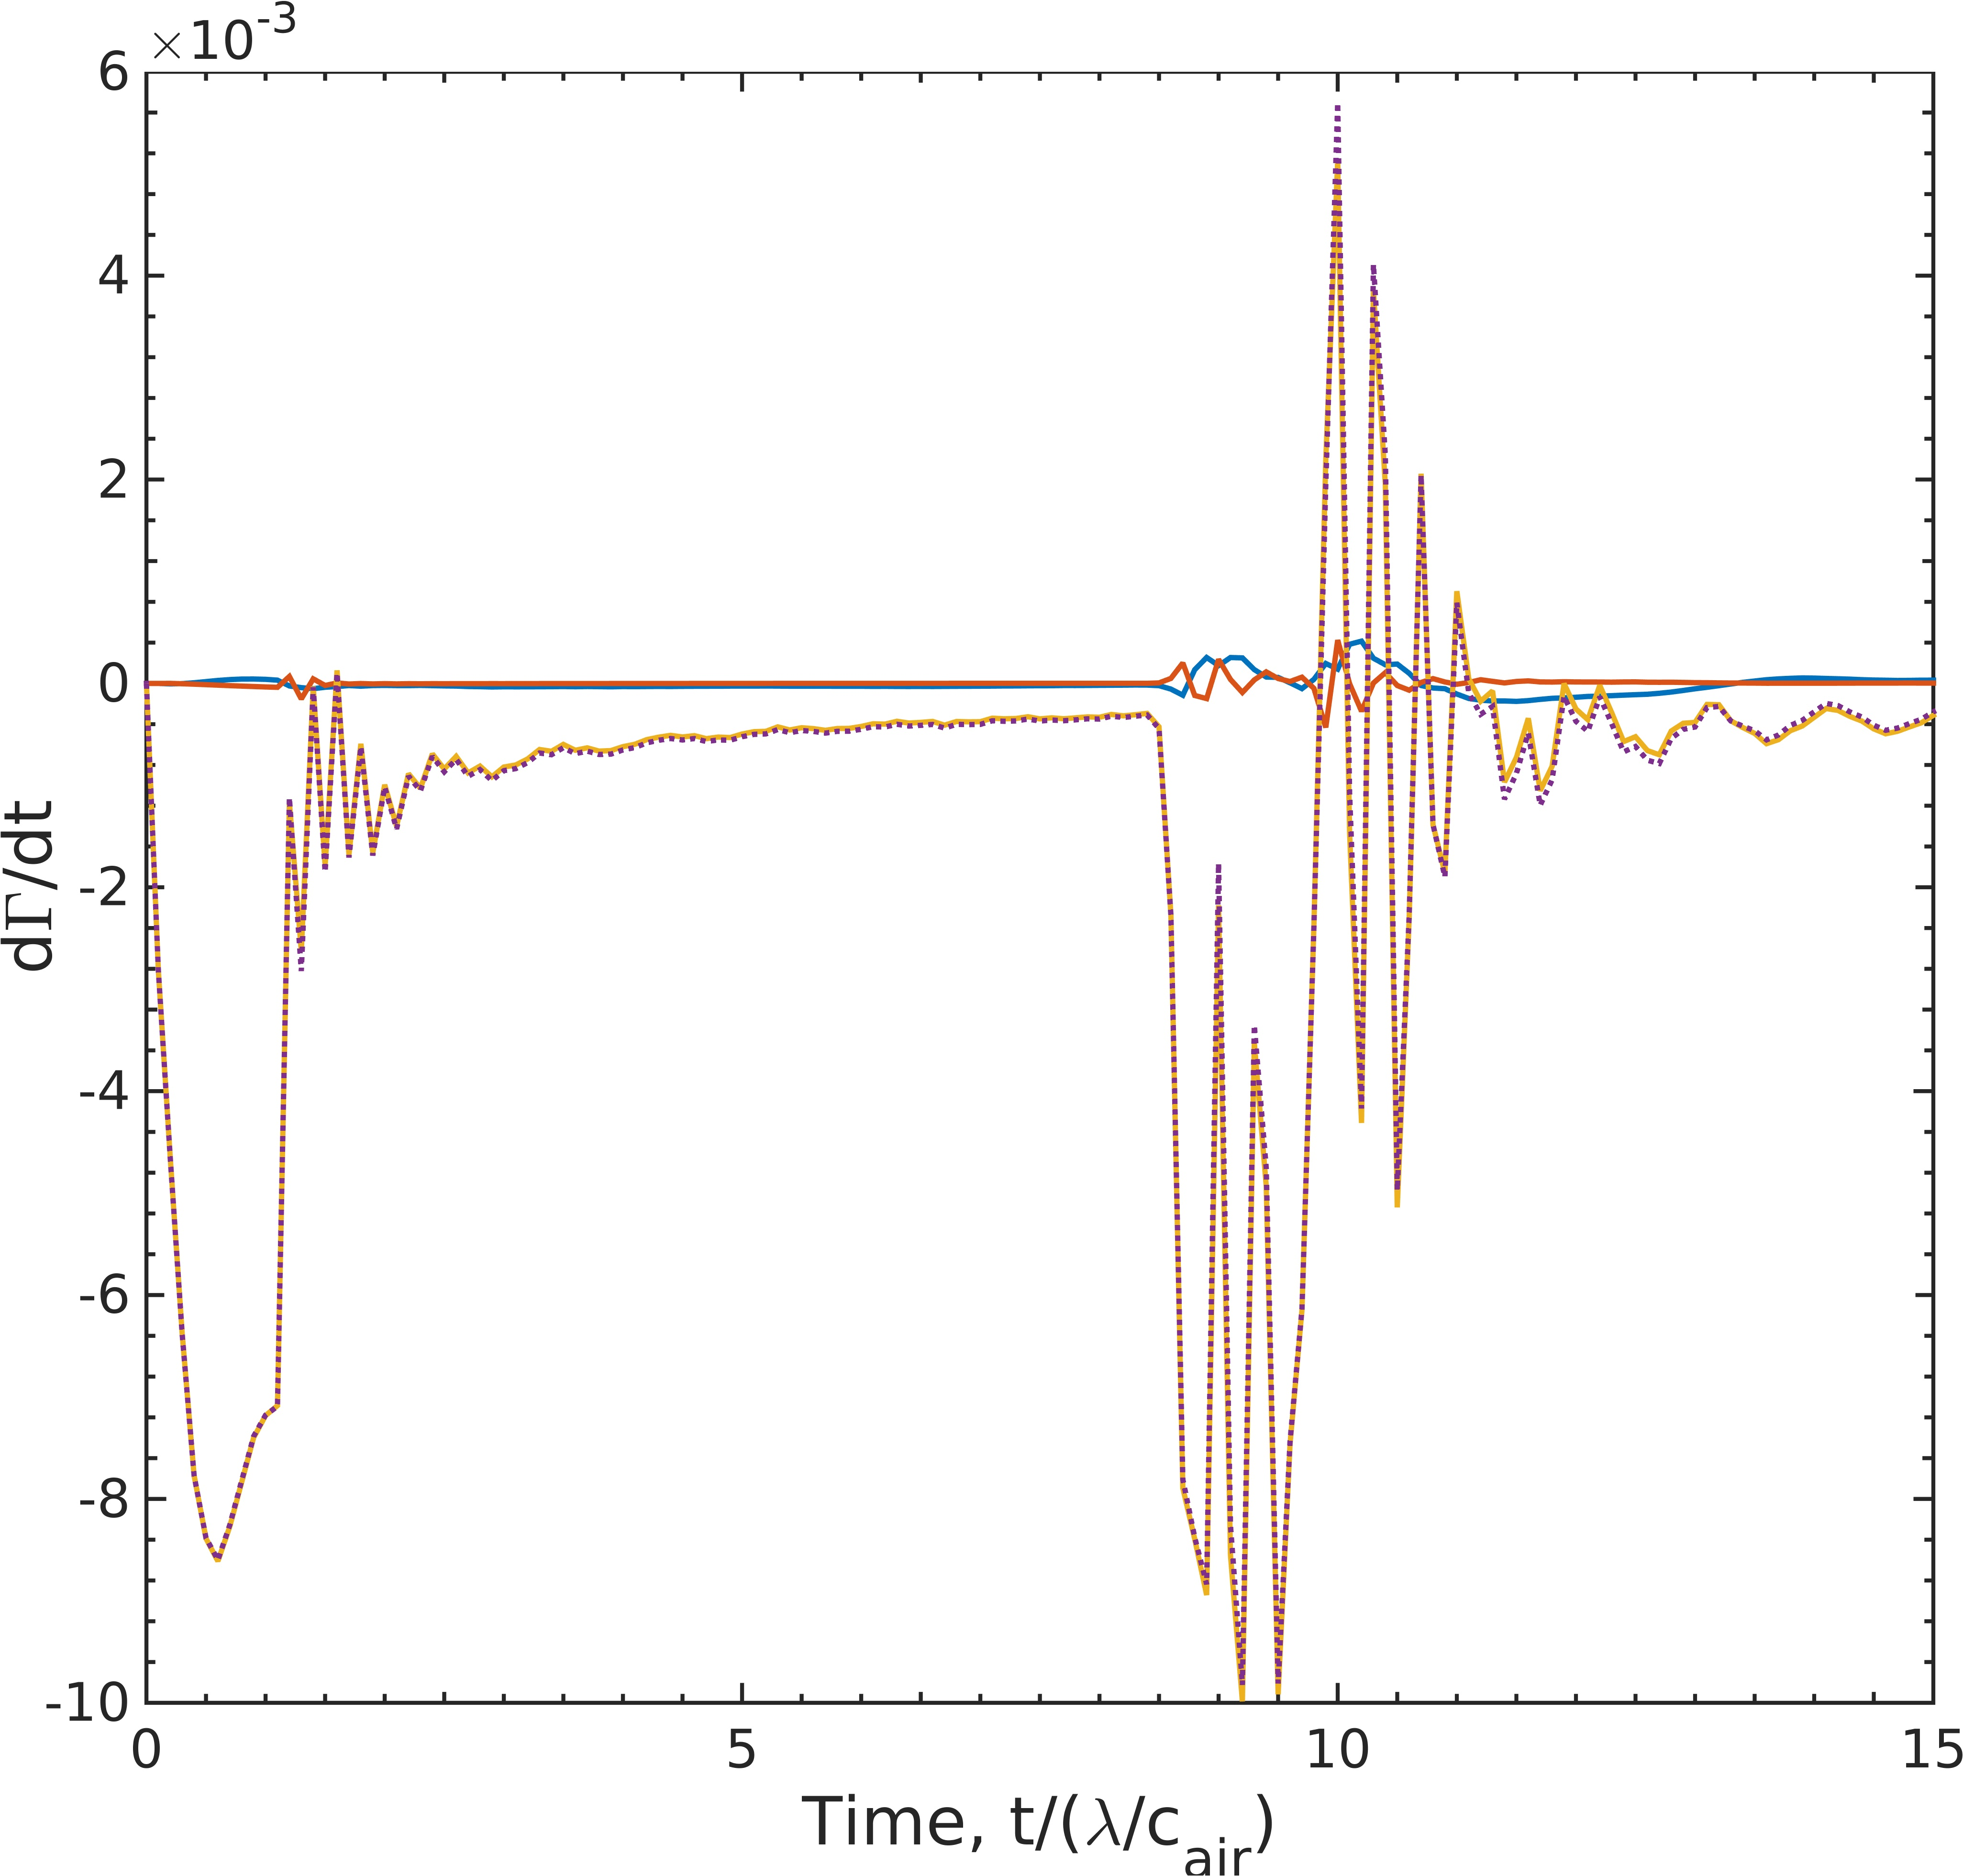
\includegraphics[width=0.48\textwidth]{./figs/lung_figs/ddtcirc}
  \caption[The vorticity field and individual contributions to circulation by physical mechanism]{A surface plot of vorticity for the $10$ MPa trapezoidal
    wave case, at time $t=0.6$, during the middle of the
    interface-compression wave interaction (Left). Each term of the
    circulation generation equation \eqref{eq:circulation_generation} is plotted as a function of time:
    $\left(d\Gamma/dt\right)_{advective}$ (blue),
    $\left(d\Gamma/dt\right)_{compressible}$ (orange),
    $\left(d\Gamma/dt\right)_{baroclinic}$ (yellow),
    $\left(d\Gamma/dt\right)_{total}$ (purple, dotted) is plotted as a
    function of time (Right).}
  \label{fig:trapz_ddt_circ}
\end{figure}
%
\subsubsection{Dependence on time-dependent wave features: time lag between compression and expansion waves}
To demonstrate the importance of time-dependent wave features, we
simulate $p_a=10$ MPa trapezoidal waves of varying duration impinging
onto the water-air interface. The compression and expansion portions
of the waveform are exactly the same as is in the other trapezoidal
wave cases, with pressure rising and falling over an initial distance
of $5\lambda$. We vary the duration of interaction between interface
and the elevated static pressure portion of the wave, we will consider
in terms of the static portion of the wave's initial length, defined
as $\Delta x_{lag}$. We decrease this duration from the typical
$\Delta x_{lag}=35\lambda$ to
$\Delta x_{lag}=25\lambda, 20\lambda, 15\lambda, 5\lambda,$ and
$0\lambda$. For each of these cases the system dynamics are virtually
identical to the original case until the expansion encounters the
interface. Figure \ref{fig:trapz_circ_interface_multi-lag} shows the
interface amplitude and circulation histories for each case. For the
three longest duration trapezoidal waves, with static elevated
pressure durations of $\Delta x_{lag}=35\lambda, 25\lambda$ and
$20\lambda$, we note that the expansion encounters the interface after
the phase reversal has already occurred. In these cases, the expansion
deposits additional circulation at the interface. For the shorter
duration waves, with static elevated pressure durations of
$\Delta x_{lag}=10\lambda, 5\lambda$ and $0\lambda$, the expansion
encounters the interface before the phase inversion and the net
half-domain circulation is decreased. We note that before or after the
phase change of the interface, the larger $a(t)$ is at the time the
expansion encounters the interface, the more circulation is generated
by the wave, though this does not necessarily hold true across the
phase inversion.
%
\begin{figure}[h] 
  \centering
  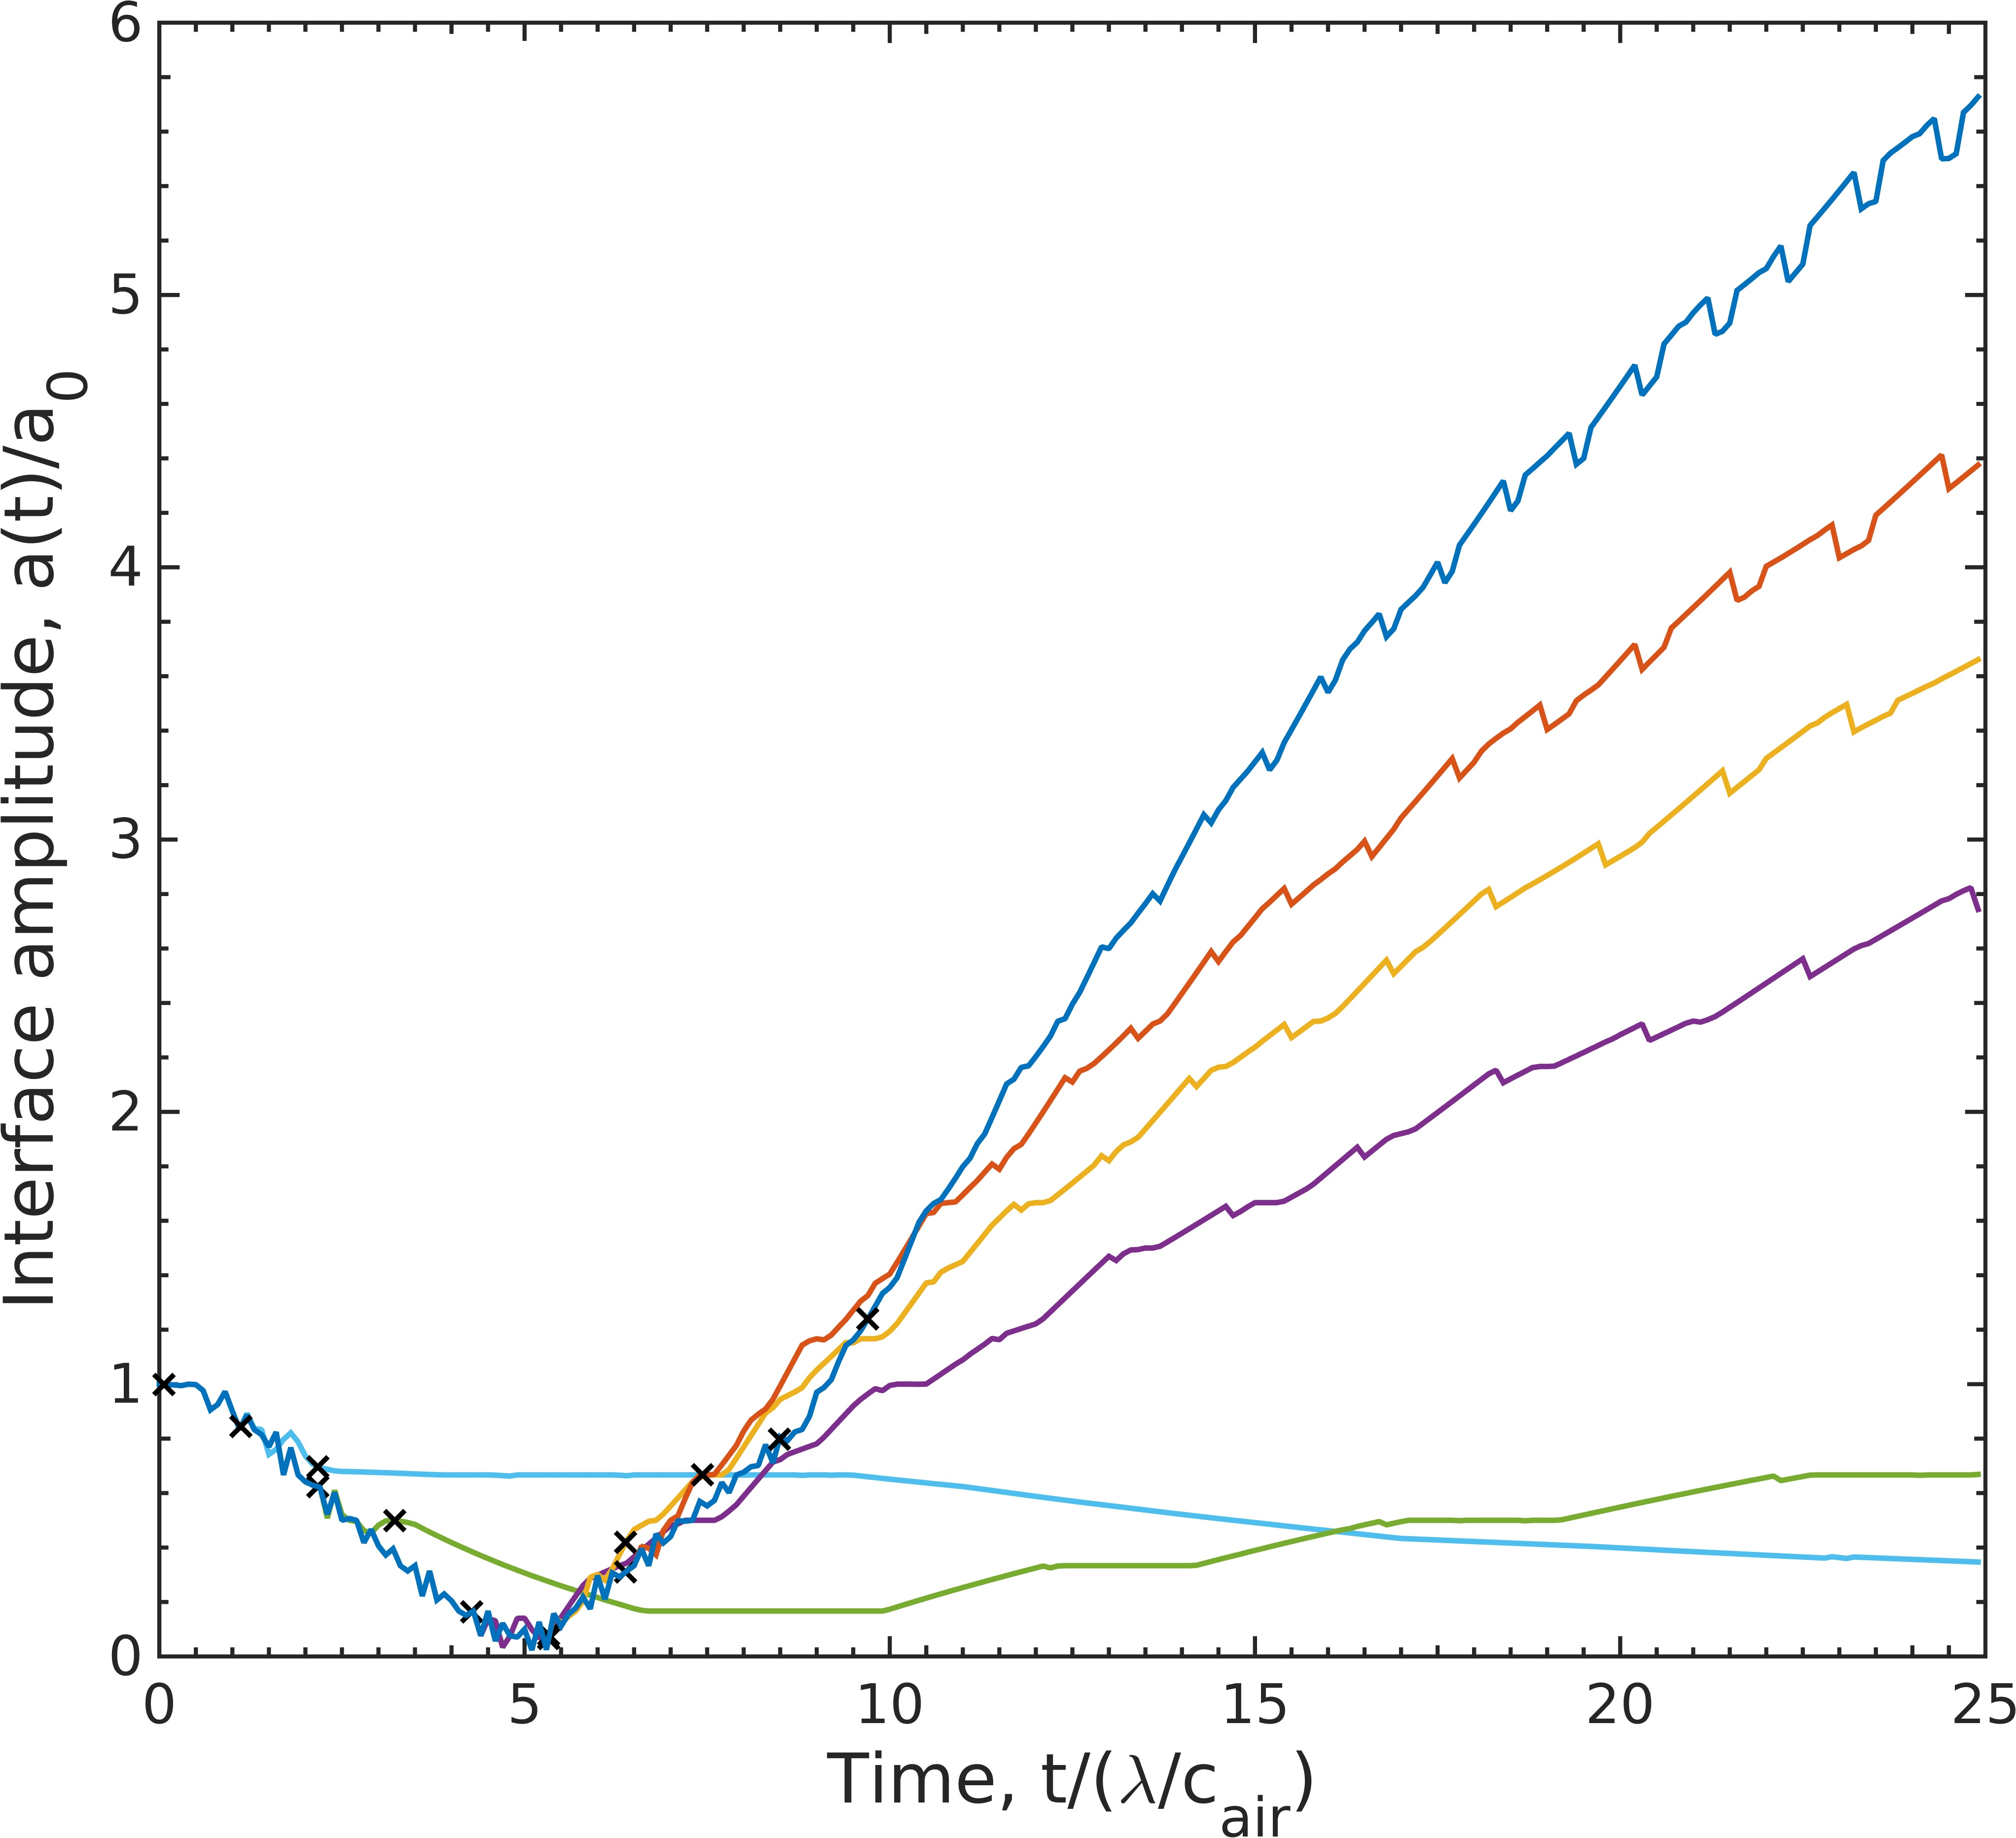
\includegraphics[width=0.48\textwidth]{./figs/lung_figs/interface_multi-lag}
  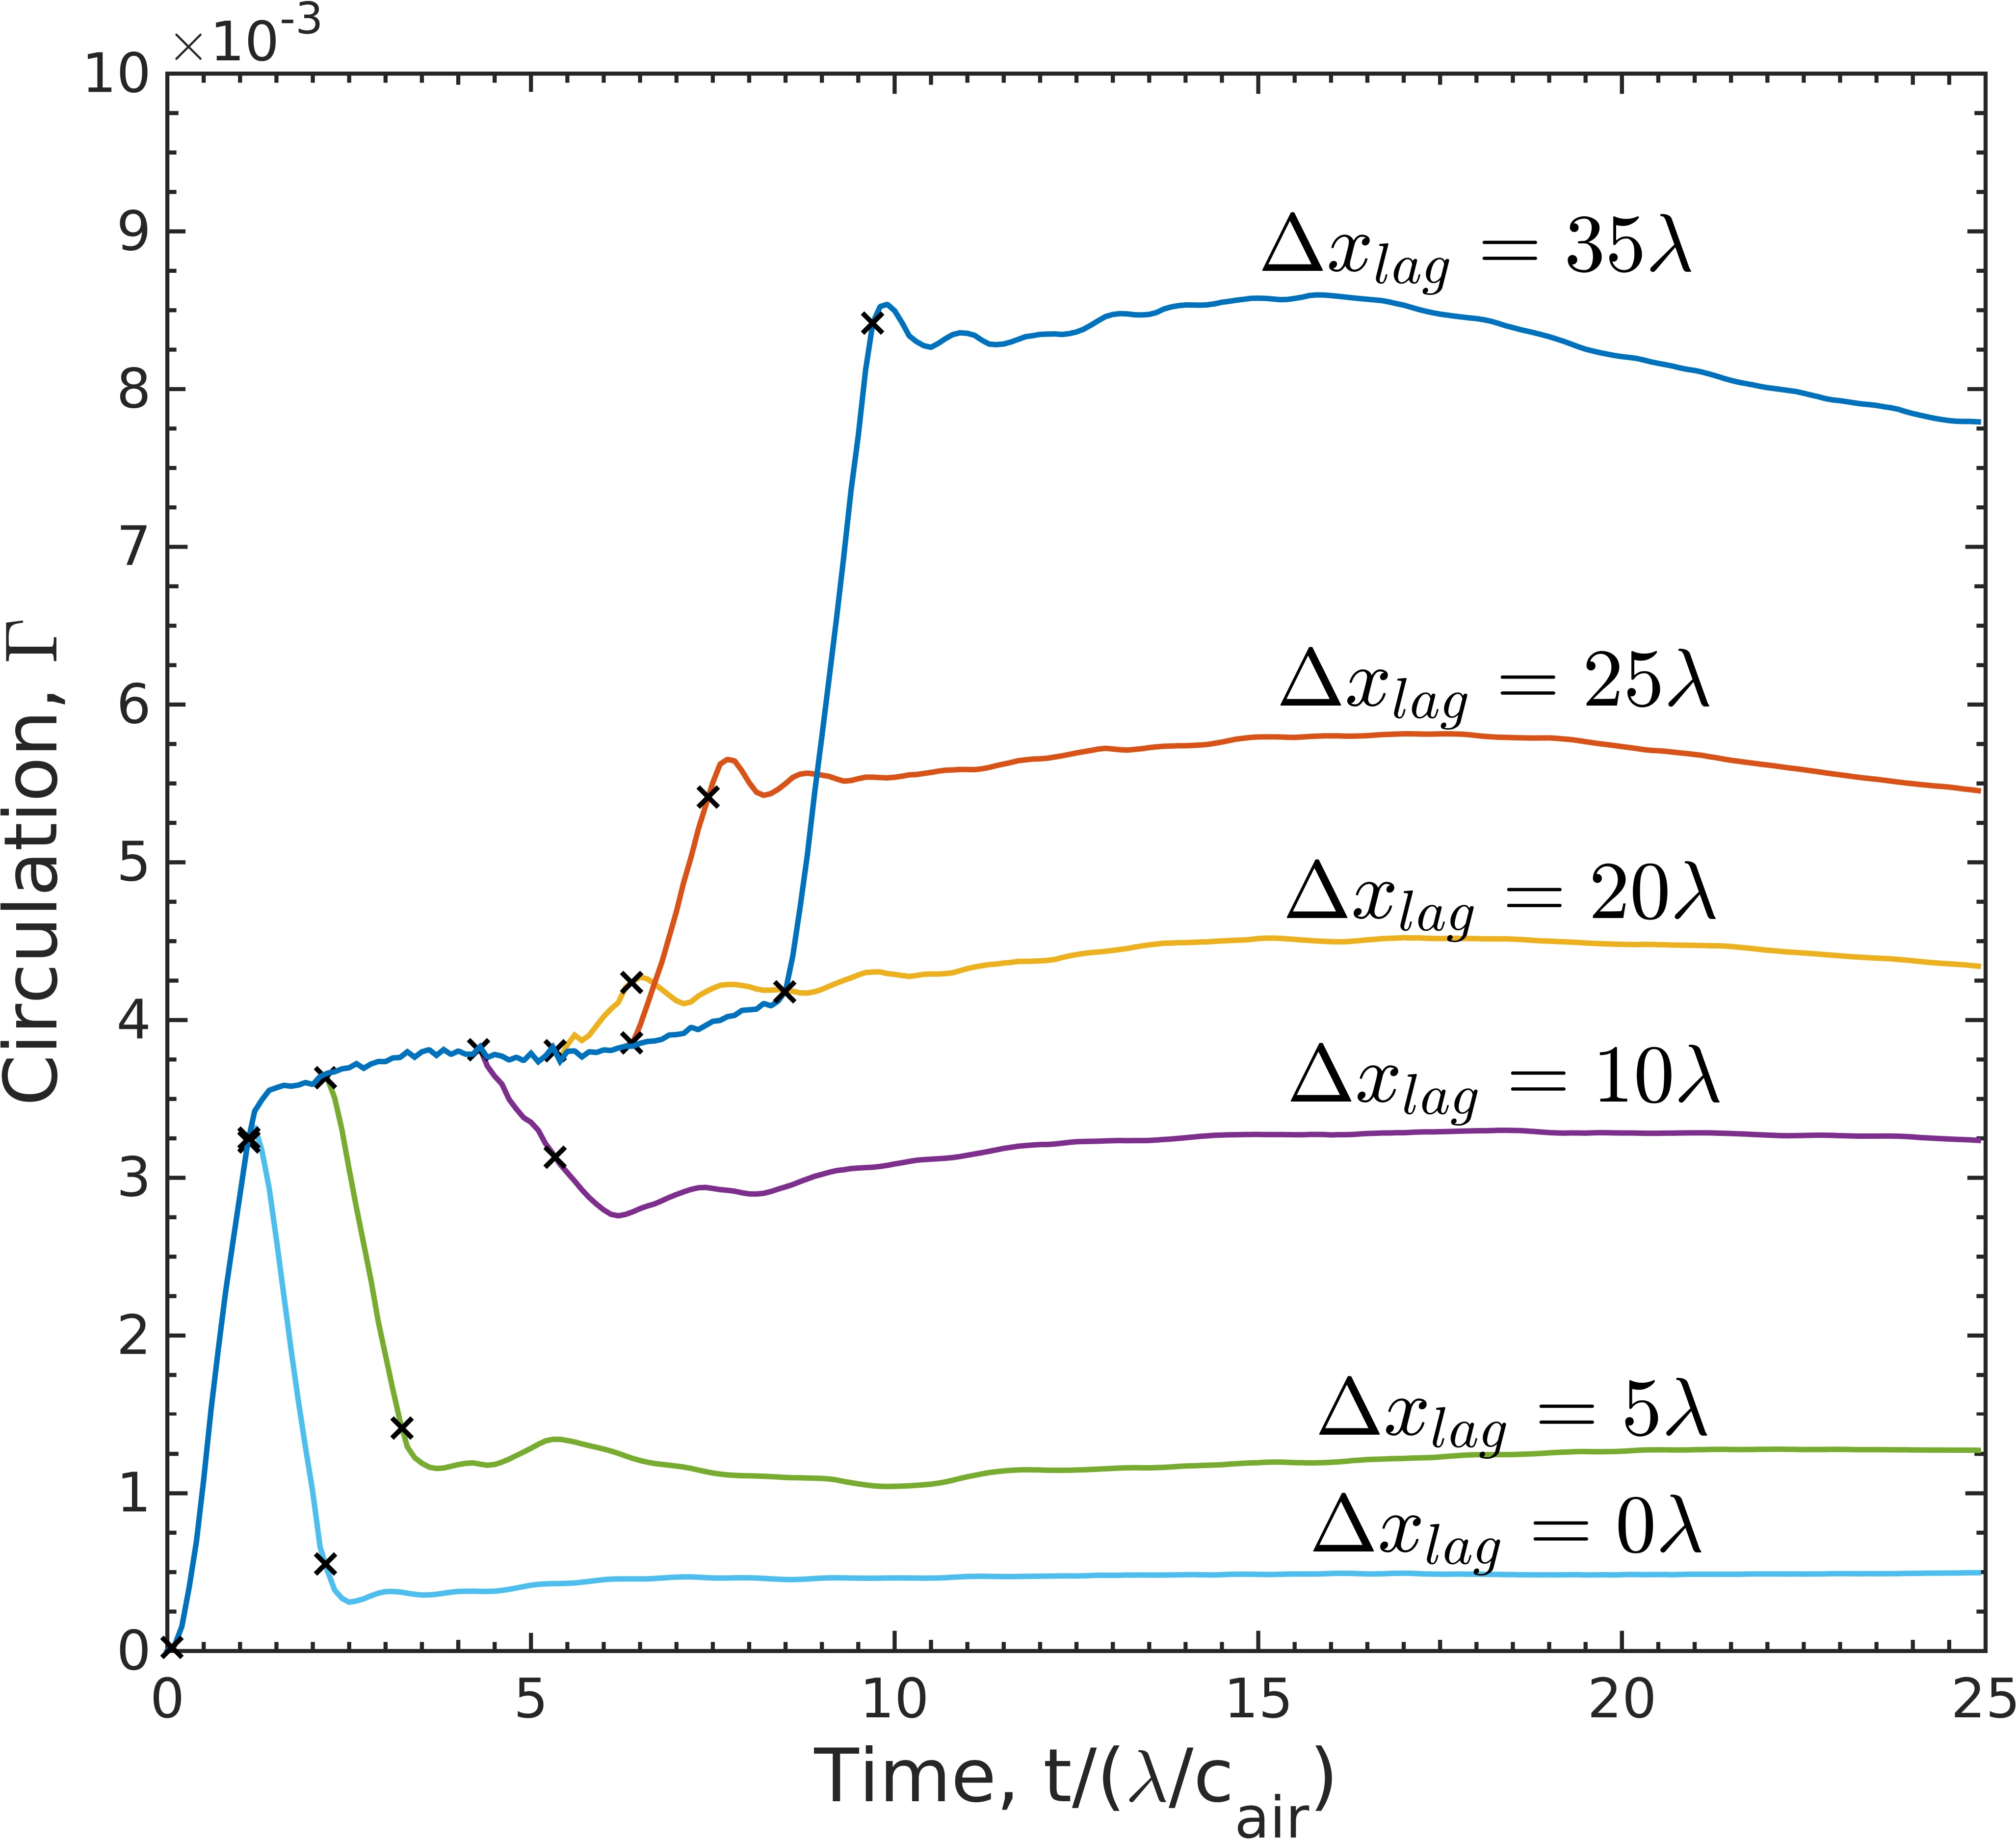
\includegraphics[width=0.48\textwidth]{./figs/lung_figs/circulation_multi-lag}
  \caption[The interface and circulation dependence on wave duration]{The interface amplitude (left) and circulation (right)
    histories for varying elevated static pressure durations or lag
    time $\Delta x_{lag}$ between the expansion and compression
    waves. Here we show results for $\Delta x_{lag}=35\lambda$ (blue),
    $\Delta x_{lag}=25\lambda$ (orange), $\Delta x_{lag}=20\lambda$
    (yellow), $\Delta x_{lag}=10\lambda$ (purple),
    $\Delta x_{lag}=5\lambda$ (green), $\Delta x_{lag}=0\lambda$
    (light blue)}
  \label{fig:trapz_circ_interface_multi-lag}
\end{figure}
%
\subsection{Interface response to \acf{DUS} waves}%
\label{subsec:usbe_lung_trapezoidal_results}%
To evaluate the relevance of our trapezoidal wave experiments we simulate
a $p_a=1, 5$ and $10$ MPa \ac{DUS} pulse waves (See Figure
\ref{fig:p0}) impinging onto the water air interface. In figure
\ref{fig:us_circ_interface} we illustrate the circulation and
interface amplitude histories for the $p_a=10$ MPa \ac{DUS} like-pulse
case. The post-wave interface dynamics are similar to those observed
for trapezoidal wave cases. During the wave-interface interaction, the
interface amplitude is compressed overall, but oscillations are
observed in correspondence with the acoustic pulse oscillations. After
the wave has left the interface, the perturbation amplitude continues
to decrease until the interface undergoes a phase inversion, after
which the perturbation amplitude grows for the remainder of the
simulation. half-domain circulation oscillates during wave-interface
interaction before settling to a nearly constant non-zero value after
the wave has passed. We note that the total circulation deposited is
of the same order of magnitude as that generated by the trapezoidal
wave of the same amplitude and duration. Qualitatively similar results
were observed for the $5$ MPa case. For the one $1$ MPa case, the
evolution of the system was slow such that running the simulation long
enough to obtain useful results was computationally prohibitive.

\begin{figure}
  \centering
  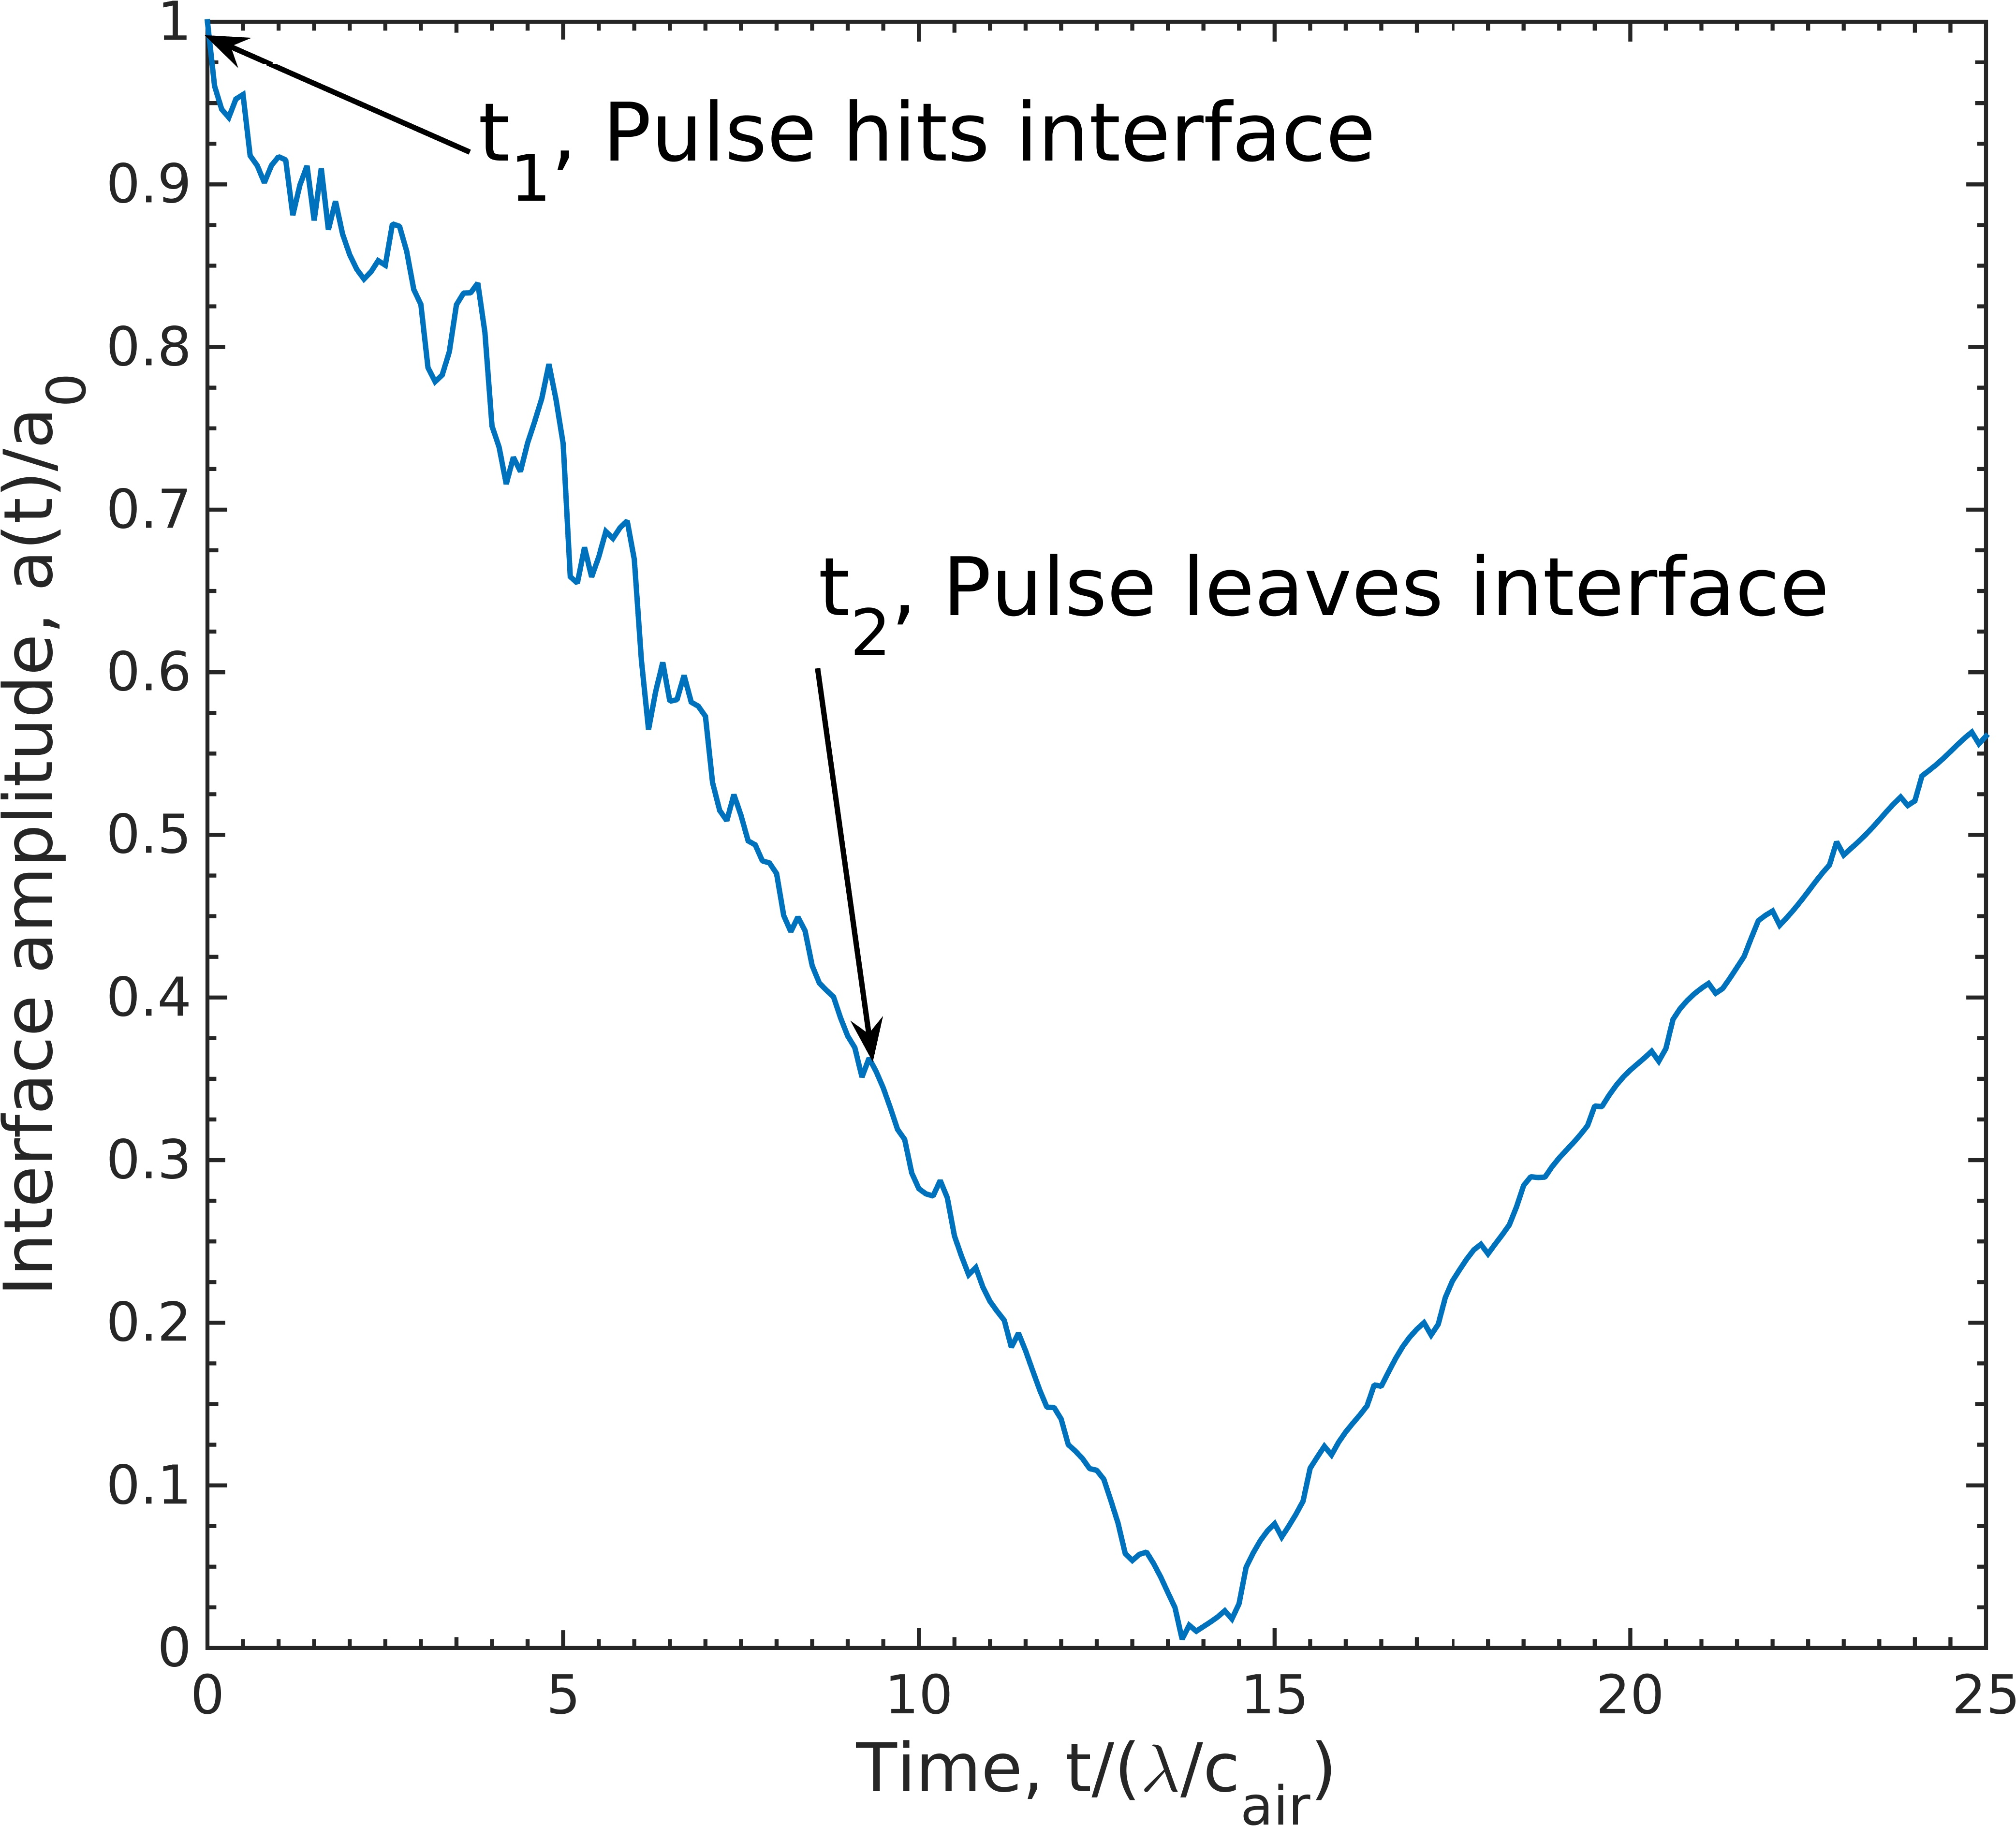
\includegraphics[width=0.48\textwidth]{./figs/lung_figs/us_intf_schematic} \hfill
  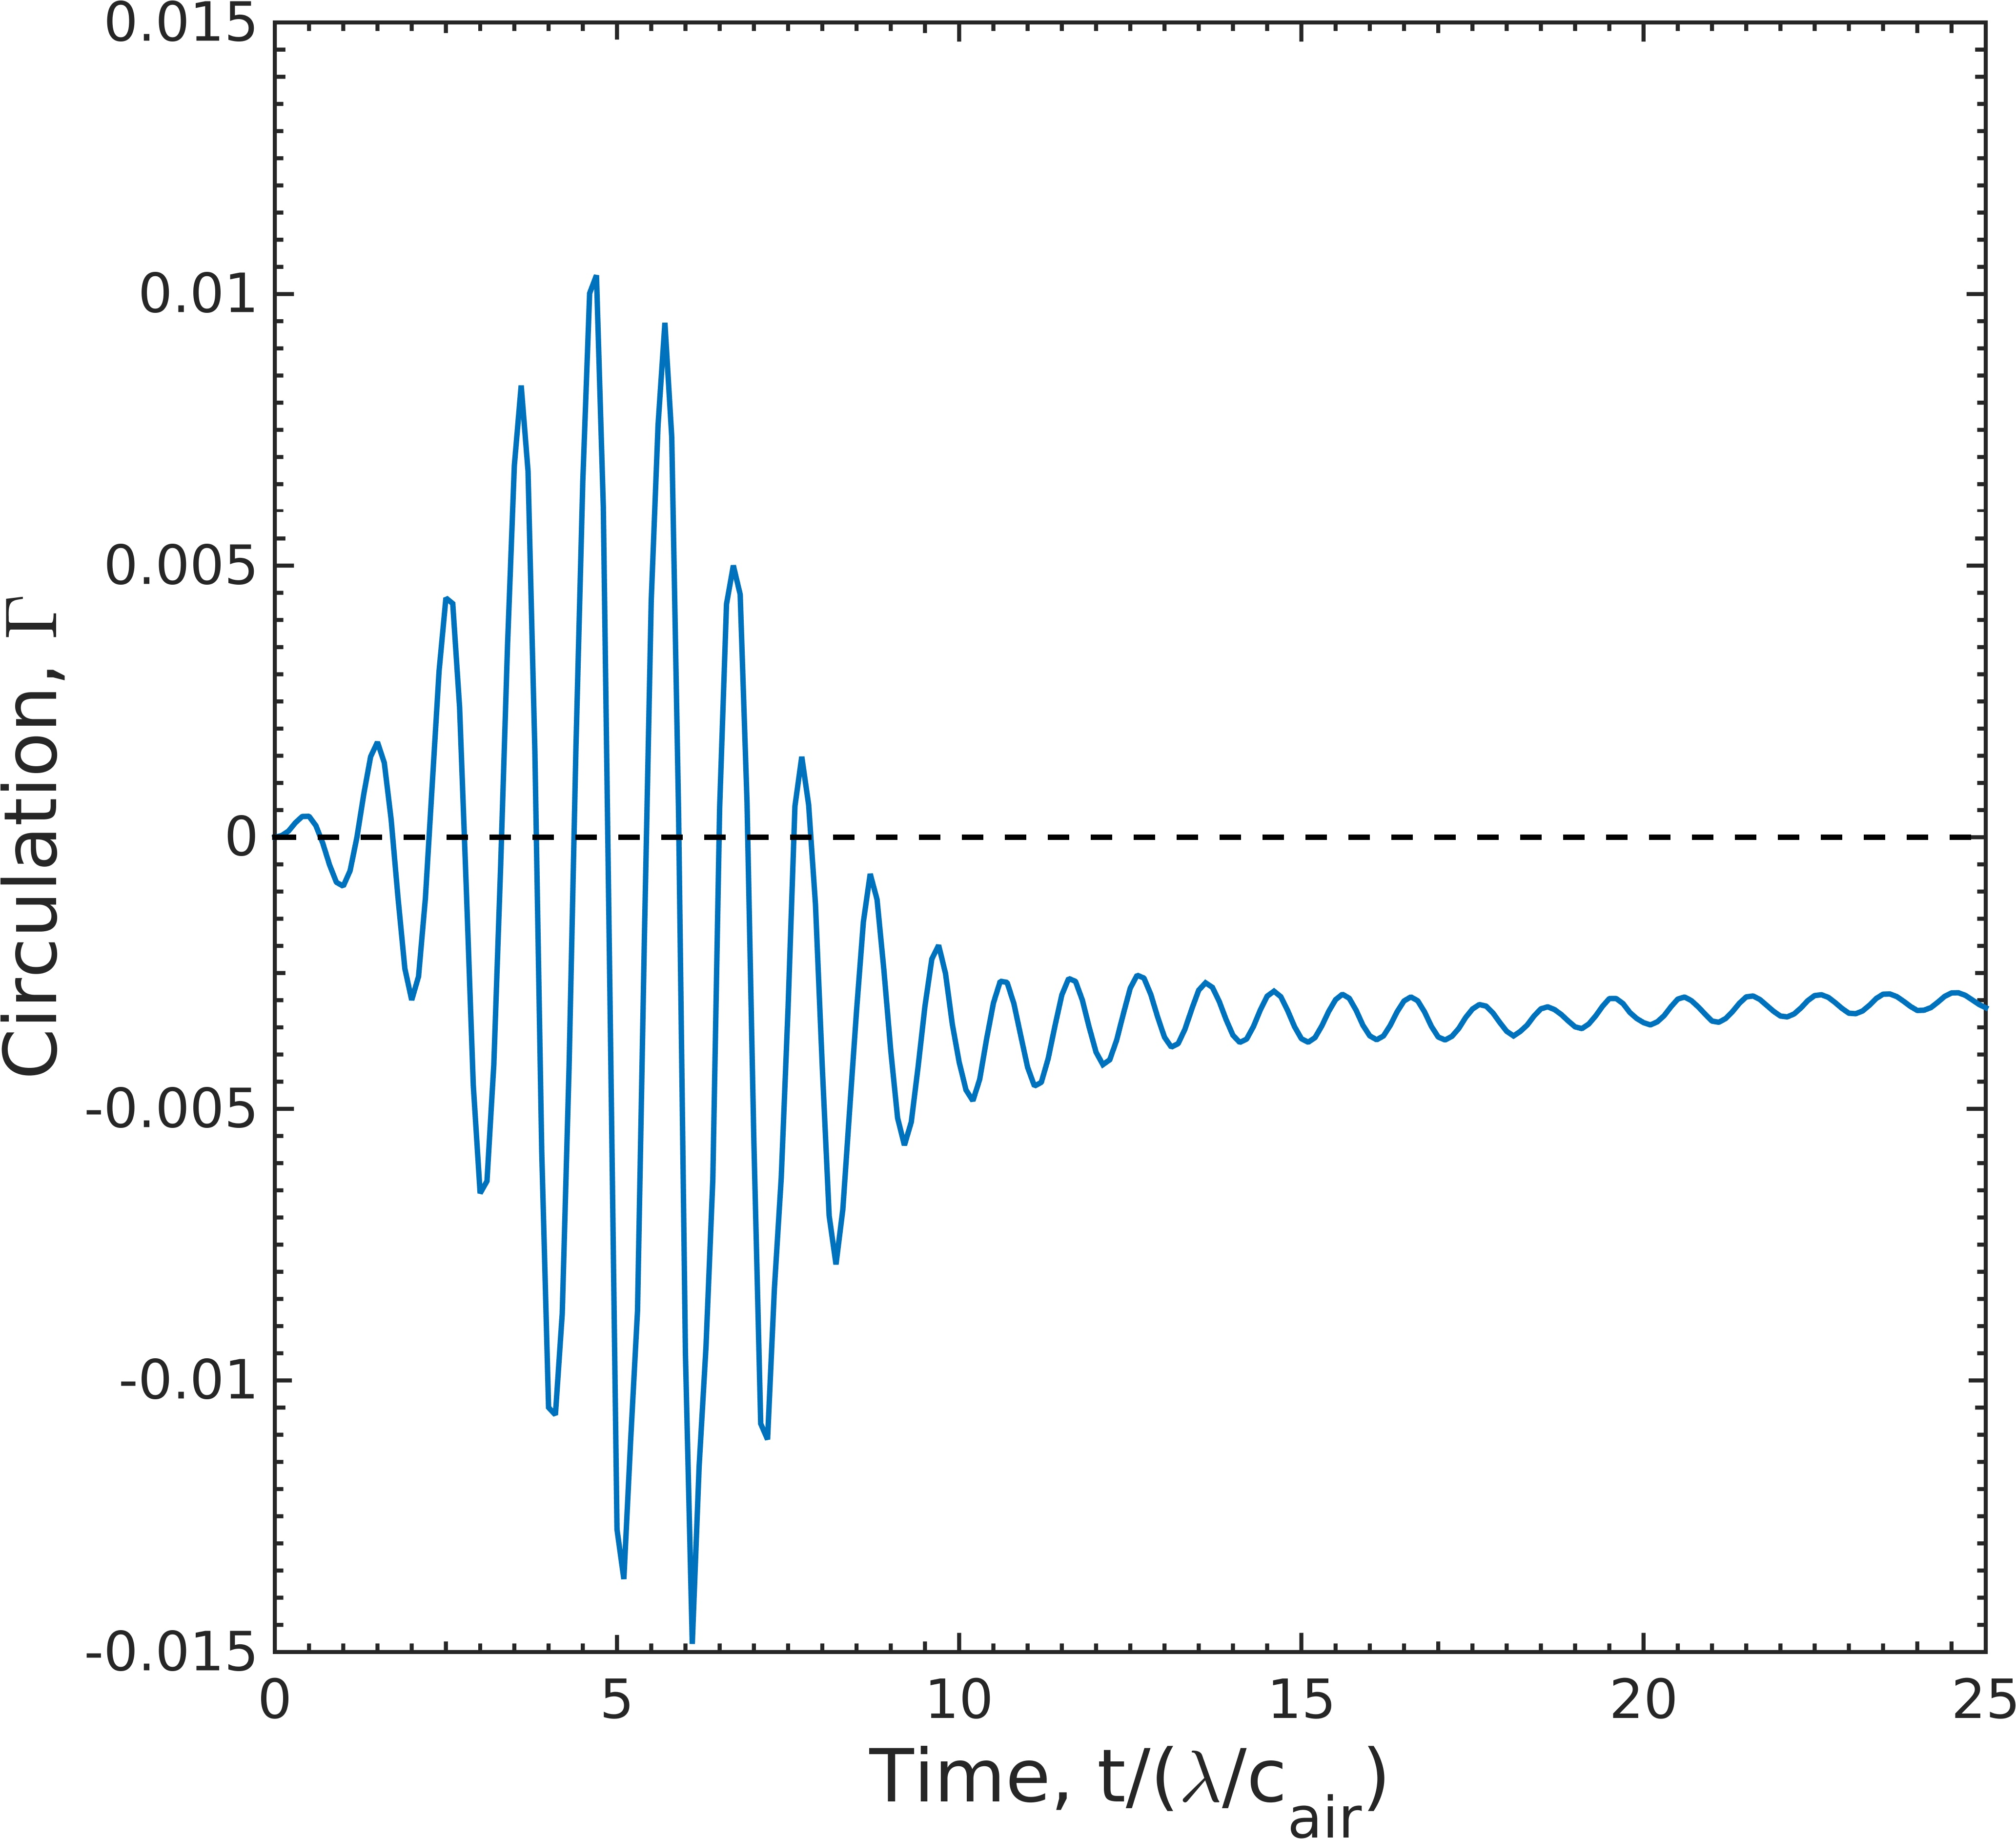
\includegraphics[width=0.48\textwidth]{./figs/lung_figs/us_circ_schematic}
  \caption[The interface amplitude and circulation histories for the \ac{DUS} pulse]{The interface amplitude (left) and circulation (right)
    histories corresponding to the a water-air interface disturbed by
    the US-like pulse shown in Figure \ref{fig:p0}.}
  \label{fig:us_circ_interface}
\end{figure}

\subsection{Further discussion of the results}%
\label{subsec:usbe_lung_further_discussion}%
For both the trapezoidal and \ac{DUS} pulse acoustic waves, the
pressure, velocity, and density return to initial, ambient conditions
after the passing of the wave. As these waveforms are continuous, this
implies that the integral of the pressure gradient $\nabla p$ at each
point along the interface, over all time must be zero. Hence we
surmise that if the interface remains unchanged during the interaction
with the wave, as it would for a wave moving with infinite velocity,
$\nabla \rho$ remains constant and the net baroclinic circulation
deposited must be zero. Thus for any finite duration acoustic wave
such as ours to deposit net baroclinic circulation upon an interface,
the interface itself must deform during interaction with the
wave. This deformation alters the misalignment of the pressure and
density gradients at the interface causing positive and negative
circulation deposited to not cancel out entirely. Note that this is
unique to waves that begin and end at the same pressure. This is not
the case for the traditional \ac{RMI} problem, for which conditions do
not return to their original state after the passage of the shock.

For the cases varying the length of the static elevated pressure in
the trapezoidal wave we previously noted that whether the expansion
increased or decreased the total half-domain circulation depended on
whether it encountered the interface before or after the phase
change. If indeed circulation is driving the deformation of the
interface, then changes in the waveform that appear to have very
little effect on the interface dynamics during the wave-interface
interaction period, may have far more significant impacts on the long
term dynamics of the interface. To put this in the context of
\ac{DUS}, which uses repeated pulses, if ultrasonically-deposited
circulation is causing deformation within the lungs, longer \acp{PD}
may allow for greater deformation and increased circulation deposition
as a result of any individual pulse. If the system acts as we have
modeled it, the \ac{PRF} would determine the degree of interface
deformation experienced by pulses subsequent to the first and may
influence deformation and hemorrhage. Finally, in recognition of the
limitations of this study, we note that the true physical nature of
lung tissue is viscoelastic \citep{Bayliss1939}, and neither viscosity
nor elasticity is included in our model problems. While preliminary
results with a Navier-Stokes code showed similar early time results,
we expect that viscosity would dissipate circulation over a long
enough period of time. Furthermore, elasticity may provide a mechanism
by which the alveolar walls could resist deformation or retard to
their original shape between pressure perturbations.




%%% Local Variables:
%%% mode: latex
%%% TeX-master: "../../prelim"
%%% End:
